% Options for packages loaded elsewhere
\PassOptionsToPackage{unicode}{hyperref}
\PassOptionsToPackage{hyphens}{url}
%
\documentclass[
  11pt,
  letterpaper,
]{scrbook}

\usepackage{amsmath,amssymb}
\usepackage{iftex}
\ifPDFTeX
  \usepackage[T1]{fontenc}
  \usepackage[utf8]{inputenc}
  \usepackage{textcomp} % provide euro and other symbols
\else % if luatex or xetex
  \usepackage{unicode-math}
  \defaultfontfeatures{Scale=MatchLowercase}
  \defaultfontfeatures[\rmfamily]{Ligatures=TeX,Scale=1}
\fi
\usepackage{lmodern}
\ifPDFTeX\else  
    % xetex/luatex font selection
\fi
% Use upquote if available, for straight quotes in verbatim environments
\IfFileExists{upquote.sty}{\usepackage{upquote}}{}
\IfFileExists{microtype.sty}{% use microtype if available
  \usepackage[]{microtype}
  \UseMicrotypeSet[protrusion]{basicmath} % disable protrusion for tt fonts
}{}
\makeatletter
\@ifundefined{KOMAClassName}{% if non-KOMA class
  \IfFileExists{parskip.sty}{%
    \usepackage{parskip}
  }{% else
    \setlength{\parindent}{0pt}
    \setlength{\parskip}{6pt plus 2pt minus 1pt}}
}{% if KOMA class
  \KOMAoptions{parskip=half}}
\makeatother
\usepackage{xcolor}
\setlength{\emergencystretch}{3em} % prevent overfull lines
\setcounter{secnumdepth}{5}
% Make \paragraph and \subparagraph free-standing
\makeatletter
\ifx\paragraph\undefined\else
  \let\oldparagraph\paragraph
  \renewcommand{\paragraph}{
    \@ifstar
      \xxxParagraphStar
      \xxxParagraphNoStar
  }
  \newcommand{\xxxParagraphStar}[1]{\oldparagraph*{#1}\mbox{}}
  \newcommand{\xxxParagraphNoStar}[1]{\oldparagraph{#1}\mbox{}}
\fi
\ifx\subparagraph\undefined\else
  \let\oldsubparagraph\subparagraph
  \renewcommand{\subparagraph}{
    \@ifstar
      \xxxSubParagraphStar
      \xxxSubParagraphNoStar
  }
  \newcommand{\xxxSubParagraphStar}[1]{\oldsubparagraph*{#1}\mbox{}}
  \newcommand{\xxxSubParagraphNoStar}[1]{\oldsubparagraph{#1}\mbox{}}
\fi
\makeatother


\providecommand{\tightlist}{%
  \setlength{\itemsep}{0pt}\setlength{\parskip}{0pt}}\usepackage{longtable,booktabs,array}
\usepackage{calc} % for calculating minipage widths
% Correct order of tables after \paragraph or \subparagraph
\usepackage{etoolbox}
\makeatletter
\patchcmd\longtable{\par}{\if@noskipsec\mbox{}\fi\par}{}{}
\makeatother
% Allow footnotes in longtable head/foot
\IfFileExists{footnotehyper.sty}{\usepackage{footnotehyper}}{\usepackage{footnote}}
\makesavenoteenv{longtable}
\usepackage{graphicx}
\makeatletter
\def\maxwidth{\ifdim\Gin@nat@width>\linewidth\linewidth\else\Gin@nat@width\fi}
\def\maxheight{\ifdim\Gin@nat@height>\textheight\textheight\else\Gin@nat@height\fi}
\makeatother
% Scale images if necessary, so that they will not overflow the page
% margins by default, and it is still possible to overwrite the defaults
% using explicit options in \includegraphics[width, height, ...]{}
\setkeys{Gin}{width=\maxwidth,height=\maxheight,keepaspectratio}
% Set default figure placement to htbp
\makeatletter
\def\fps@figure{htbp}
\makeatother
% definitions for citeproc citations
\NewDocumentCommand\citeproctext{}{}
\NewDocumentCommand\citeproc{mm}{%
  \begingroup\def\citeproctext{#2}\cite{#1}\endgroup}
\makeatletter
 % allow citations to break across lines
 \let\@cite@ofmt\@firstofone
 % avoid brackets around text for \cite:
 \def\@biblabel#1{}
 \def\@cite#1#2{{#1\if@tempswa , #2\fi}}
\makeatother
\newlength{\cslhangindent}
\setlength{\cslhangindent}{1.5em}
\newlength{\csllabelwidth}
\setlength{\csllabelwidth}{3em}
\newenvironment{CSLReferences}[2] % #1 hanging-indent, #2 entry-spacing
 {\begin{list}{}{%
  \setlength{\itemindent}{0pt}
  \setlength{\leftmargin}{0pt}
  \setlength{\parsep}{0pt}
  % turn on hanging indent if param 1 is 1
  \ifodd #1
   \setlength{\leftmargin}{\cslhangindent}
   \setlength{\itemindent}{-1\cslhangindent}
  \fi
  % set entry spacing
  \setlength{\itemsep}{#2\baselineskip}}}
 {\end{list}}
\usepackage{calc}
\newcommand{\CSLBlock}[1]{\hfill\break\parbox[t]{\linewidth}{\strut\ignorespaces#1\strut}}
\newcommand{\CSLLeftMargin}[1]{\parbox[t]{\csllabelwidth}{\strut#1\strut}}
\newcommand{\CSLRightInline}[1]{\parbox[t]{\linewidth - \csllabelwidth}{\strut#1\strut}}
\newcommand{\CSLIndent}[1]{\hspace{\cslhangindent}#1}

% \usepackage{amsmath,amssymb,mathtools}
\usepackage{enumerate}
\usepackage{geometry}
\geometry{hmargin=1.2in}

\usepackage{booktabs}
\usepackage{amssymb}
\makeatletter
\def\thm@space@setup{%
  \thm@preskip=8pt plus 2pt minus 4pt
  \thm@postskip=\thm@preskip
}
\makeatother

\usepackage{framed,color}
\definecolor{shadecolor}{RGB}{248,248,248}

\renewcommand{\textfraction}{0.05}
\renewcommand{\topfraction}{0.8}
\renewcommand{\bottomfraction}{0.8}
\renewcommand{\floatpagefraction}{0.75}

%\let\oldhref\href
%\renewcommand{\href}[2]{#2\footnote{\url{#1}}}

\ifxetex
  \usepackage{letltxmacro}
  \setlength{\XeTeXLinkMargin}{1pt}
  \LetLtxMacro\SavedIncludeGraphics\includegraphics
  \def\includegraphics#1#{% #1 catches optional stuff (star/opt. arg.)
    \IncludeGraphicsAux{#1}%
  }%
  \newcommand*{\IncludeGraphicsAux}[2]{%
    \XeTeXLinkBox{%
      \SavedIncludeGraphics#1{#2}%
    }%
  }%
\fi

\makeatletter
\newenvironment{kframe}{%
\medskip{}
\setlength{\fboxsep}{.8em}
 \def\at@end@of@kframe{}%
 \ifinner\ifhmode%
  \def\at@end@of@kframe{\end{minipage}}%
  \begin{minipage}{\columnwidth}%
 \fi\fi%
 \def\FrameCommand##1{\hskip\@totalleftmargin \hskip-\fboxsep
 \colorbox{shadecolor}{##1}\hskip-\fboxsep
     % There is no \\@totalrightmargin, so:
     \hskip-\linewidth \hskip-\@totalleftmargin \hskip\columnwidth}%
 \MakeFramed {\advance\hsize-\width
   \@totalleftmargin\z@ \linewidth\hsize
   \@setminipage}}%
 {\par\unskip\endMakeFramed%
 \at@end@of@kframe}
\makeatother

\makeatletter
\@ifundefined{Shaded}{
}{\renewenvironment{Shaded}{\begin{kframe}}{\end{kframe}}}
\makeatother

\newenvironment{rmdblock}[1]
  {
  \begin{itemize}
  \renewcommand{\labelitemi}{
    \raisebox{-.7\height}[0pt][0pt]{
      {\setkeys{Gin}{width=3em,keepaspectratio}\includegraphics{images/#1}}
    }
  }
  \setlength{\fboxsep}{1em}
  \begin{kframe}
  \item
  }
  {
  \end{kframe}
  \end{itemize}
  }
\newenvironment{rmdnote}
  {\begin{rmdblock}{note}}
  {\end{rmdblock}}
\newenvironment{rmdcaution}
  {\begin{rmdblock}{caution}}
  {\end{rmdblock}}
\newenvironment{rmdimportant}
  {\begin{rmdblock}{important}}
  {\end{rmdblock}}
\newenvironment{rmdtip}
  {\begin{rmdblock}{tip}}
  {\end{rmdblock}}
\newenvironment{rmdwarning}
  {\begin{rmdblock}{warning}}
  {\end{rmdblock}}
\usepackage{mathrsfs}
\DeclareMathAlphabet{\mathcrl}{U}{rsfs}{m}{n}
\usepackage{utopia}
\DeclareMathAlphabet{\mathcal}{OMS}{cmsy}{m}{n}
\usepackage{pdfpages}
\usepackage{booktabs}
\usepackage{longtable}
\usepackage{array}
\usepackage{multirow}
\usepackage{wrapfig}
\usepackage{float}
\usepackage{colortbl}
\usepackage{pdflscape}
\usepackage{tabu}
\usepackage{threeparttable}
\usepackage{threeparttablex}
\usepackage[normalem]{ulem}
\usepackage{makecell}
\usepackage{xcolor}
\makeatletter
\@ifpackageloaded{bookmark}{}{\usepackage{bookmark}}
\makeatother
\makeatletter
\@ifpackageloaded{caption}{}{\usepackage{caption}}
\AtBeginDocument{%
\ifdefined\contentsname
  \renewcommand*\contentsname{Table des matières}
\else
  \newcommand\contentsname{Table des matières}
\fi
\ifdefined\listfigurename
  \renewcommand*\listfigurename{Liste des figures}
\else
  \newcommand\listfigurename{Liste des figures}
\fi
\ifdefined\listtablename
  \renewcommand*\listtablename{Liste des tableaux}
\else
  \newcommand\listtablename{Liste des tableaux}
\fi
\ifdefined\figurename
  \renewcommand*\figurename{Figure}
\else
  \newcommand\figurename{Figure}
\fi
\ifdefined\tablename
  \renewcommand*\tablename{Tableau}
\else
  \newcommand\tablename{Tableau}
\fi
}
\@ifpackageloaded{float}{}{\usepackage{float}}
\floatstyle{ruled}
\@ifundefined{c@chapter}{\newfloat{codelisting}{h}{lop}}{\newfloat{codelisting}{h}{lop}[chapter]}
\floatname{codelisting}{Énumération}
\newcommand*\listoflistings{\listof{codelisting}{Liste des énumérations}}
\usepackage{amsthm}
\theoremstyle{definition}
\newtheorem{example}{Exemple}[chapter]
\theoremstyle{definition}
\newtheorem{definition}{Définition}[chapter]
\theoremstyle{remark}
\AtBeginDocument{\renewcommand*{\proofname}{Preuve}}
\newtheorem*{remark}{Remarque}
\newtheorem*{solution}{Solution}
\newtheorem{refremark}{Remarque}[chapter]
\newtheorem{refsolution}{Solution}[chapter]
\makeatother
\makeatletter
\makeatother
\makeatletter
\@ifpackageloaded{caption}{}{\usepackage{caption}}
\@ifpackageloaded{subcaption}{}{\usepackage{subcaption}}
\makeatother

\ifLuaTeX
\usepackage[bidi=basic]{babel}
\else
\usepackage[bidi=default]{babel}
\fi
\babelprovide[main,import]{french}
% get rid of language-specific shorthands (see #6817):
\let\LanguageShortHands\languageshorthands
\def\languageshorthands#1{}
\ifLuaTeX
  \usepackage{selnolig}  % disable illegal ligatures
\fi
\usepackage{bookmark}

\IfFileExists{xurl.sty}{\usepackage{xurl}}{} % add URL line breaks if available
\urlstyle{same} % disable monospaced font for URLs
\hypersetup{
  pdftitle={MATH 60604 - Modélisation statistique},
  pdfauthor={Léo Belzile},
  pdflang={fr},
  hidelinks,
  pdfcreator={LaTeX via pandoc}}


\title{MATH 60604 - Modélisation statistique}
\author{Léo Belzile}
\date{2024-08-21}

\begin{document}

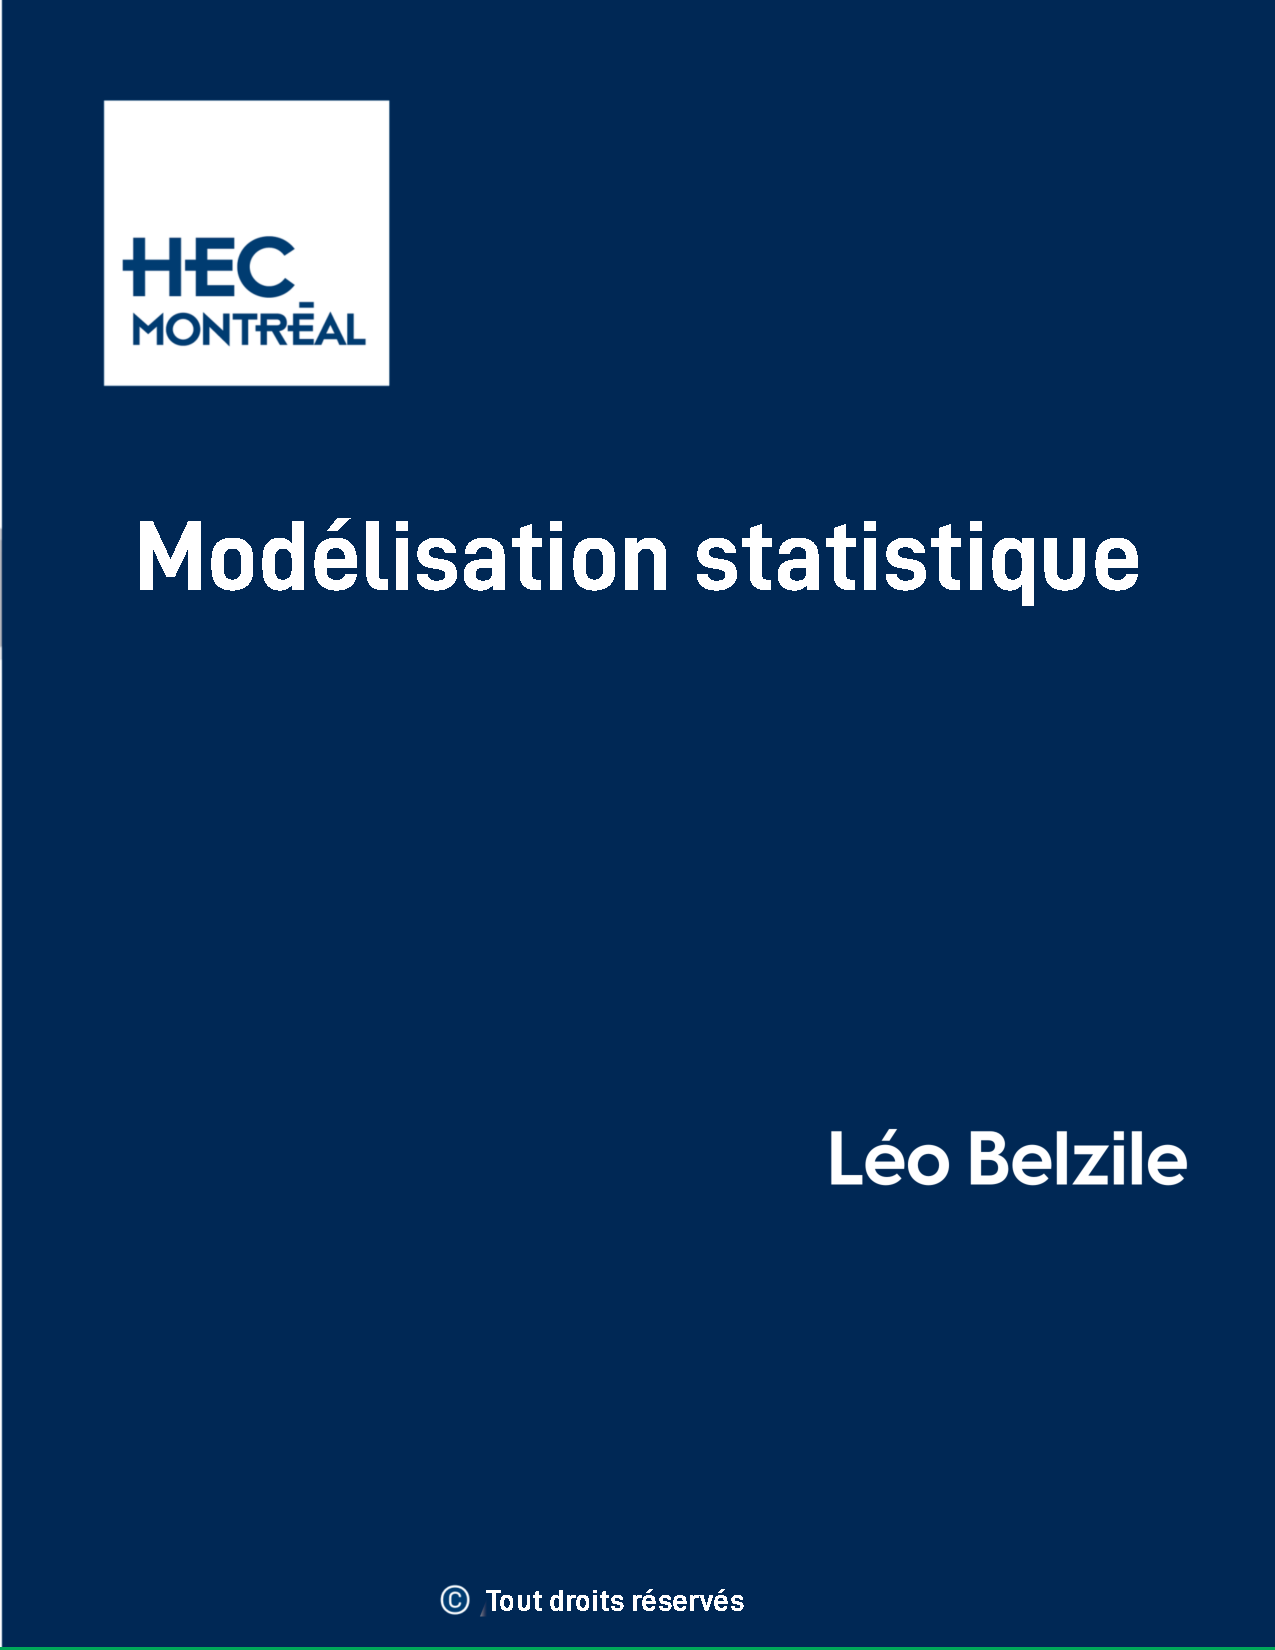
\includepdf{figures/coverpage.pdf}

\renewcommand*\contentsname{Table des matières}
{
\setcounter{tocdepth}{2}
\tableofcontents
}

\mainmatter
\bookmarksetup{startatroot}

\chapter*{Bienvenue}\label{bienvenue}
\addcontentsline{toc}{chapter}{Bienvenue}

\markboth{Bienvenue}{Bienvenue}

Ces notes sont l'oeuvre de Léo Belzile (HEC Montréal) et sont mises à
disposition sous la
\href{https://creativecommons.org/licenses/by-nc-sa/4.0/legalcode.fr}{Licence
publique Creative Commons Attribution - Utilisation non commerciale -
Partage dans les mêmes conditions 4.0 International}.

Ce cours traite de modélisation des données. Une citation célèbre
attribuée à George Box dit que

\begin{quote}
tous les modèles sont faux, mais certains sont utiles.
\end{quote}

Ce point de vue est réducteur; McCullagh et Nelder
(\citeproc{ref-McCullagh.Nelder:1989}{1989}) (traduction libre)
expliquent dans le préambule de leur livre

\begin{quote}
La modélisation en science demeure, du moins partiellement, un art.
Certains principes existent, en revanche, pour guider le modélisateur.
Le premier est que tous les modèles sont faux; mais que \textbf{certains
sont meilleurs} et \textbf{le modélisateur doit chercher le meilleur à
sa portée}. En même temps, il est sage de reconnaître que la quête
perpétuelle de la vérité n'est pas envisageable.
\end{quote}

Et David R. Cox (traduction libre), de rajouter

\begin{quote}
\ldots il n'est pas utile de simplement énoncer que tout modèle est
faux. L'idée même de modèle sous-tend une notion de simplification et
d'idéalisation. L'idée qu'un système physique, biologique ou
sociologique complexe puisse être décrit de manière exacte par quelques
formules est franchement absurde. La construction de
\textbf{représentations idéalisées qui capturent les aspects stables les
plus importants du système} est néanmoins une partie essentielle de
toute analyse scientifique et les modèles statistiques ne diffèrent pas
en cela d'autres types de modèles.
\end{quote}

Pourquoi utiliser des modèles?
\href{https://krugman.blogs.nytimes.com/2010/11/18/debt-deleveraging-and-the-liquidity-trap/}{Paul
Krugman écrivait en 2010 dans son blogue}

\begin{quote}
La réponse que je donnerais est que les modèles sont un outil énormément
important pour clarifier ses pensées. Vous n'avez pas à avoir une foi
aveugle en votre modèle {[}\ldots{]} pour croire qu'en mettant sur pied
une description simplifiée, mais complète du fonctionnement du système
{[}\ldots{]} vous permet de gagner une compréhension plus sophistiquée
de la situation réelle. Les personnes qui n'utilisent pas de modèles
finissent par se baser sur des slogans beaucoup plus simplistes que les
modèles.
\end{quote}

\section*{Contenu du cours}\label{contenu-du-cours}
\addcontentsline{toc}{section}{Contenu du cours}

\markright{Contenu du cours}

L'inférence statistique a pour but de tirer des conclusions formelles à
partir de données. Dans le cadre de la recherche scientifique, le
chercheur formule une hypothèse, collecte des données et conclut quant à
la plausibilité de son hypothèse.

On distingue deux types de jeux de données: les données
\textbf{expérimentales} sont typiquement collectées en milieu contrôlé
suivant un protocole d'enquête et un plan d'expérience: elles servent à
répondre à une question prédéterminée. L'approche expérimentale est
désirable pour éviter le «jardin des embranchements» (une
\href{http://www.stat.columbia.edu/~gelman/research/unpublished/p_hacking.pdf}{allégorie
signifiant qu'un chercheur peut raffiner son hypothèse à la lumière des
données, sans ajustement pour des variables confondantes}), mais elle
n'est pas toujours réalisable: par exemple, un économiste ne peut pas
modifier les taux d'intérêts pour observer les impacts sur le taux
d'épargne des consommateurs. Lorsque les données ont été collectées
préalablement à d'autres fins, on parle de données
\textbf{observationnelles}.

Par modèle, on entendra la spécification d'une loi aléatoire pour les
données et une équation reliant les paramètres ou l'espérance
conditionnelle d'une variable réponse \(Y\) à un ensemble de variables
explicatives \(\mathbf{X}\). Ce modèle peut servir à des fins de
prédiction (modèle prédictif) ou pour tester des hypothèses de recherche
concernant les effets de ces variables (modèle explicatif). Ces deux
objectifs ne sont pas mutuellement exclusifs même si on fait parfois une
distinction entre inférence et prédiction.

Un modèle prédictif permet d'obtenir des prédictions de la valeur de
\(Y\) pour d'autres combinaisons de variables explicatives ou des
données futures. Par exemple, on peut chercher à prédire la consommation
énergétique d'une maison en fonction de la météo, du nombre d'habitants
de la maison et de sa taille. La plupart des boîtes noires utilisées en
apprentissage automatique tombent dans la catégorie des modèles
prédictifs: ces modèles ne sont pas interprétables et ignorent parfois
la structure inhérente aux données.

Par contraste, les modèles explicatifs sont souvent simples et
interprétables, et les modèles de régressions sont fréquemment utilisés
pour l'inférence. On se concentrera dans ce cours sur les modèles
explicatifs. Par exemple, on peut chercher à déterminer

\begin{itemize}
\tightlist
\item
  Est-ce que les décisions intégrées (décision combinée d'achat et de
  quantité) sont préférables aux décisions séquentielles (décision
  d'acheter, puis choix de la quantité) lors de l'achat d'un produit en
  ligne (\citeproc{ref-Duke.Amir:2023}{Duke et Amir 2023})?
\item
  Qu'est-ce qui est le plus distrayant pour les utilisateurs de la
  route: parler au cellulaire, texter en conduisant, consulter sa montre
  intelligente (\citeproc{ref-Brodeur:2021}{Brodeur et al. 2021})?
\item
  Quel est l'impact de de l'inadéquation entre l'image d'un produit et
  sa description (\citeproc{ref-Lee.Choi:2019}{Lee et Choi 2019})?
\item
  Qu'est-ce qui explique que les prix de l'essence soient plus élevés en
  Gaspésie qu'ailleurs au Québec?
  \href{http://www.regie-energie.qc.ca/energie/rapports/Rapport_PrixGasp\%C3\%A9sie_20191219.pdf}{Un
  rapport de surveillance des prix de l'essence en Gaspésie par la Régie
  de l'énergie se penche sur la question.}
\item
  Est-ce que les examens pratiques de conduite en Grande-Bretagne sont
  plus faciles dans les régions à faible densité?
  \href{https://www.theguardian.com/world/2019/aug/23/an-easy-ride-scottish-village-fuels-debate-driving-test-pass-rates}{Une
  analyse du journal britannique \emph{The Guardian}} laisse penser que
  c'est le cas.
\item
  Quelle est la perception environnementale d'un emballage de carton
  (versus de plastique) s'il englobe un contenant en plastique
  (\citeproc{ref-Sokolova:2023}{Sokolova, Krishna, et Döring 2023}).
\item
  Quel est l'impact psychologique des suggestions sur le montant de dons
  (\citeproc{ref-Moon.VanEpps:2023}{Moon et VanEpps 2023})?
\item
  Est-ce que la visioconférence réduit le nombre d'interactions et
  d'idée créatives générées lors d'une réunion, par rapport à une
  rencontre en personne (\citeproc{ref-Brucks.Levav:2022}{Brucks et
  Levav 2022})?
\end{itemize}

\bookmarksetup{startatroot}

\chapter{Introduction}\label{intro}

\section{Rappels}\label{rappels}

Ce chapitre couvre des rappels mathématiques de probabilité et
statistique d'ordinaire couverts dans un cours de niveau collégial ou
préuniversitaire.

\subsection{Population et échantillons}\label{population-echantillon}

Ce qui différencie la statistique des autres sciences est la prise en
compte de l'incertitude et de la notion d'aléatoire. Règle générale, on
cherche à estimer une caractéristique d'une population définie à l'aide
d'un échantillon (un sous-groupe de la population) de taille restreinte.

La \textbf{population d'intérêt} est un ensemble d'individus formant la
matière première d'une étude statistique. Par exemple, pour l'Enquête
sur la population active (EPA) de Statistique Canada, « la population
cible comprend la population canadienne civile non institutionnalisée de
15 ans et plus ». Même si on faisait un recensement et qu'on
interrogeait tous les membres de la population cible, la caractéristique
d'intérêt peut varier selon le moment de la collecte; une personne peut
trouver un emploi, quitter le marché du travail ou encore se retrouver
au chômage. Cela explique la variabilité intrinsèque.

En général, on se base sur un \textbf{échantillon} pour obtenir de
l'information parce que l'acquisition de données est coûteuse.
L'\textbf{inférence statistique} vise à tirer des conclusions, pour
toute la population, en utilisant seulement l'information contenue dans
l'échantillon et en tenant compte des sources de variabilité. Le sondeur
George Gallup (traduction libre) a fait cette merveilleuse analogie
entre échantillon et population:

\begin{quote}
«Il n'est pas nécessaire de manger un bol complet de soupe pour savoir
si elle est trop salé; pour autant qu'elle ait été bien brassée, une
cuillère suffit.»
\end{quote}

Un \textbf{échantillon} est un sous-groupe d'individus de la population.
Si on veut que ce dernier soit représentatif, il devrait être tiré
aléatoirement de la population, ce qui nécessite une certaine
connaissance de cette dernière. Au siècle dernier, les bottins
téléphoniques pouvaient servir à créer des plans d'enquête. C'est un
sujet complexe et des cours entiers d'échantillonnage y sont consacrés.
Même si on ne collectera pas de données, il convient de noter la
condition essentielle pour pouvoir tirer des conclusions fiables à
partir d'un échantillon: ce dernier doit être représentatif de la
population étudiée, en ce sens que sa composition doit être similaire à
celle de la population, et aléatoire. On doit ainsi éviter les biais de
sélection, notamment les échantillons de commodité qui consistent en une
sélection d'amis et de connaissances.

Si notre échantillon est \textbf{aléatoire}, notre mesure d'une
caractéristique d'intérêt le sera également et la conclusion de notre
procédure de test variera d'un échantillon à l'autre. Plus la taille de
ce dernier est grande, plus on obtiendra une mesure précise de la
quantité d'intérêt. L'exemple suivant illustre pourquoi le choix de
l'échantillon est important.

\begin{example}[Gallup et l'élection présidentielle américaine de
1936]\protect\hypertarget{exm-Gallup}{}\label{exm-Gallup}

Désireuse de prédire le résultat de l'élection présidentielle américaine
de 1936, la revue \emph{Literary Digest} a sondé 10 millions d'électeurs
par la poste, dont 2.4 millions ont répondu au sondage en donnant une
nette avance au candidat républicain Alf Landon (57\%) face au président
sortant Franklin D. Roosevelt (43\%). Ce dernier a néanmoins remporté
l'élection avec 62\% des suffrages, une erreur de prédiction de 19\%. Le
plan d'échantillonnage avait été conçu en utilisant des bottins
téléphoniques, des enregistrements d'automobiles et des listes de
membres de clubs privés, etc.:
\href{https://www.jstor.org/stable/2749114}{la non-réponse
différentielle et un échantillon biaisé} vers les classes supérieures
sont en grande partie responsable de cette erreur.

Gallup avait de son côté correctement prédit la victoire de Roosevelt en
utilisant un échantillon aléatoire de (seulement) 50 000 électeurs. Vous
pouvez lire
l'\href{https://ozanozbey.medium.com/two-lessons-of-sampling-bias-from-1936-us-election-e4e96bd42be}{histoire
complète (en anglais)}.

\end{example}

\subsection{Types de variables}\label{types-de-variables}

Le résultat d'une collecte de données est un tableau, ou base de
données, contenant sur chaque ligne des observations et en colonne des
variables. Le Tableau~\ref{tbl-data-renfe} donne un exemple de
structure.

\begin{itemize}
\tightlist
\item
  Une \textbf{variable} représente une caractéristique de la population
  d'intérêt, par exemple le sexe d'un individu, le prix d'un article,
  etc.
\item
  une \textbf{observation}, parfois appelée donnée, est un ensemble de
  mesures collectées sous des conditions identiques, par exemple pour un
  individu ou à un instant donné.
\end{itemize}

\begin{longtable}[]{@{}rllllrl@{}}

\caption{\label{tbl-data-renfe}Premières lignes de la base de données
\texttt{renfe}, qui contient les prix de 10K billets de train entre
Barcelone et Madrid.}

\tabularnewline

\toprule\noalign{}
prix & type & classe & tarif & dest & duree & jour \\
\midrule\noalign{}
\endhead
\bottomrule\noalign{}
\endlastfoot
143.4 & AVE & Preferente & Promo & Barcelone-Madrid & 190 & 6 \\
181.5 & AVE & Preferente & Flexible & Barcelone-Madrid & 190 & 2 \\
86.8 & AVE & Preferente & Promo & Barcelone-Madrid & 165 & 7 \\
86.8 & AVE & Preferente & Promo & Barcelone-Madrid & 190 & 7 \\
69.0 & AVE-TGV & Preferente & Promo & Barcelone-Madrid & 175 & 4 \\

\end{longtable}

Le choix de modèle statistique ou de test dépend souvent du type de
variables collectées. Les variables peuvent être de plusieurs types:
quantitatives (discrètes ou continues) si elles prennent des valeurs
numériques, qualitatives (binaires, nominales ou ordinales) si elles
peuvent être décrites par un adjectif; je préfère le terme catégorielle,
plus évocateur.

Les modèles de régression servent à expliquer des variables
quantitatives en fonction d'autres caractéristiques.

\begin{itemize}
\tightlist
\item
  une variable discrète prend un nombre dénombrable de valeurs; ce sont
  souvent des variables de dénombrement ou des variables dichotomiques.
\item
  une variable continue peut prendre (en théorie) une infinité de
  valeurs, même si les valeurs mesurées sont arrondies ou mesurées avec
  une précision limitée (temps, taille, masse, vitesse, salaire). Dans
  bien des cas, nous pouvons considérer comme continues des variables
  discrètes si elles prennent un assez grand nombre de valeurs.
\end{itemize}

Les variables catégorielles représentent un ensemble fini de
possibilités. On les regroupe en deux types, pour lesquels on ne fera
pas de distinction:

\begin{itemize}
\tightlist
\item
  nominales s'il n'y a pas d'ordre entre les modalités (sexe, couleur,
  pays d'origine) ou
\item
  ordinale (échelle de Likert, tranche salariale).
\end{itemize}

La codification des modalités des variables catégorielle est arbitraire;
en revanche, on préservera l'ordre lorsqu'on représentera graphiquement
les variables ordinales. Lors de l'estimation, chaque variable
catégorielle doit est transformée en un ensemble d'indicateurs binaires
0/1: il est donc essentiel de déclarer ces dernières dans votre logiciel
statistique, surtout si elles sont parfois encodées dans la base de
données à l'aide de valeurs entières.

\subsection{Variables aléatoires}\label{variable-aleatoire}

Suppsons qu'on cherche à décrire le comportement d'un phénomène
aléatoire. Pour ce faire, on cherche à décrire l'ensemble des valeurs
possibles et leur probabilité/fréquence relative au sein de la
population: ces dernières sont encodées dans la loi de la variable
aléatoire.

On fera la distinction entre deux cas de figure: quand le phénomène
prend des valeurs finies et dénombrables, comme par exemple un événement
binaire (achat/non-achat d'un produit) ou d'une variable de décompte, on
parle de distribution \textbf{discrète}. Si l'ensemble des valeurs que
prend la variable d'intérêt est dans un continuum de valeurs (par
exemple, le prix d'un item, même si en pratique il y aura une
sous-division finie et que le montant sera arrondi au centime près pour
l'argent), on parle de variable \textbf{continue}. Des cas plus
complexes peuvent survenir.

On dénote les variables aléatoires par des lettres majuscules, et leurs
réalisations par des minuscules: par exemple,
\(Y \sim \mathsf{normale}(\mu, \sigma^2)\) indique que \(Y\) suit une
loi normale de paramètres \(\mu \in \mathbb{R}\) et \(\sigma > 0\). On
parle de famille de lois si la valeur des paramètres ne sont pas
spécifiées; si on fixe plutôt ces dernière, on obtient une
représentation qui encode les probabilité.

\begin{definition}[Fonctions de répartition, de masse et de
densité]\protect\hypertarget{def-repartition}{}\label{def-repartition}

La \textbf{fonction de répartition} \(F(y)\) donne la probabilité
cumulative qu'un événement n'excède pas une variable donnée,
\(F(y) = \mathsf{Pr}(Y \leq y)\). Si la variable \(Y\) prend des valeurs
discrètes, alors on utilise la \textbf{fonction de masse}
\(f(y)=\mathsf{Pr}(Y=y)\) qui donne la probabilité pour chacune des
valeurs de \(y\). Si la variable \(Y\) est continue, aucune valeur
numérique de \(y\) n'a de probabilité non-nulle et \(\Pr(Y=y) = 0\) pour
toute valeur réelle \(y\); la \textbf{densité}, aussi dénotée \(f(x)\),
est une fonction est non-négative et satisfait
\(\int_{\mathbb{R}} f(x) \mathrm{d}x=1\): elle décrit la probabilité
d'obtenir un résultat dans un ensemble donné des réels \(\mathbb{R}\),
pour n'importe lequel intervalle. La densité sert à estimer la
probabilité que la variable continue \(Y\) appartienne à un ensemble
\(B\), via \(\mathsf{Pr}(Y \in B) = \int_B f(y) \mathrm{d} y\); la
fonction de répartition est ainsi définie comme
\(F(y) = \int_{-\infty}^y f(x) \mathrm{d} x\).

\begin{figure}[ht!]

\centering{

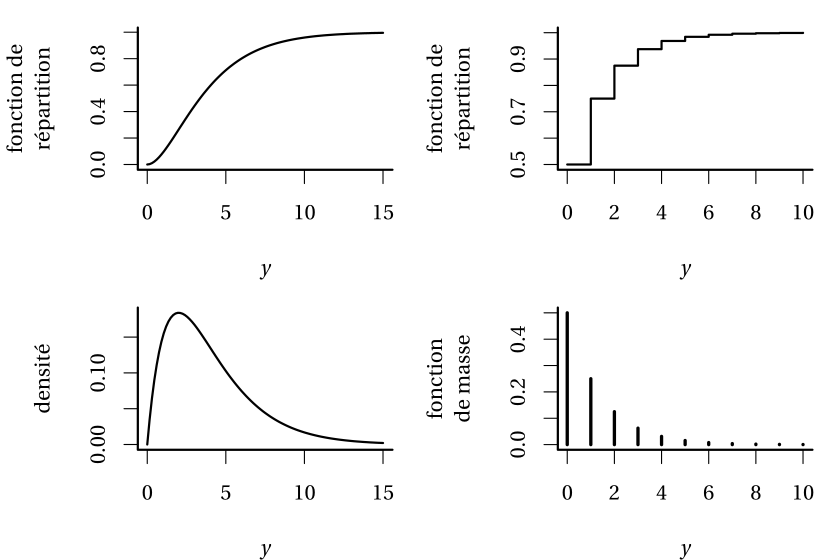
\includegraphics[width=0.85\textwidth,height=\textheight]{images/02-ttest-DF_illustration_fr.png}

}

\caption{\label{fig-distributions}Fonctions de répartition (panneau
supérieur) et fonctions de densité et de masse (panneau inférieur) pour
une loi continue (gauche) et discrète (droite).}

\end{figure}%

\end{definition}

Un premier cours de statistique débute souvent par la présentation de
statistiques descriptives comme la moyenne et l'écart-type. Ce sont des
estimateurs des moments (centrés), qui caractérisent la loi du phénomène
d'intérêt. Dans le cas de la loi normale unidimensionnelle, qui a deux
paramètres, l'espérance et la variance caractérisent complètement le
modèle.

\begin{definition}[Moments]\protect\hypertarget{def-moments}{}\label{def-moments}

Soit \(Y\) une variable aléatoire de fonction de densité (ou de masse)
\(f(x)\). On définit l'espérance d'une variable aléatoire \(Y\) comme
\begin{align*}
\mathsf{E}(Y)=\int_{\mathbb{R}} y f(y) \mathrm{d} y.
\end{align*} L'espérance est la « moyenne théorique», ou moment de
premier ordre : dans le cas discret,
\(\mu = \mathsf{E}(Y)=\sum_{y \in \mathcal{y}} y \mathsf{Pr}(y=y)\), où
\(\mathcal{Y}\) représente le support de la loi, à savoir les valeurs
qui peuvent prendre \(Y\). Plus généralement, l'espérance d'une fonction
\(g(y)\) pour une variable aléatoire \(Y\) est simplement l'intégrale de
\(g(y)\) pondérée par la densité \(f(y)\). De même, si l'intégrale est
convergente, la \textbf{variance} est \begin{align*}
\mathsf{Va}(Y)&=\int_{\mathbb{R}} (y-\mu)^2 f(y) \mathrm{d} y \\&=\mathsf{E}\{Y-\mathsf{E}(Y)\}^2 \\&= \mathsf{E}(Y^2) - \{\mathsf{E}(Y)\}^2.
\end{align*}

\end{definition}

\begin{definition}[Biais]\protect\hypertarget{def-biais}{}\label{def-biais}

Le biais d'un estimateur \(\hat{\theta}\) pour un paramètre \(\theta\)
est \begin{align*}
\mathsf{biais}(\hat{\theta})=\mathsf{E}(\hat{\theta})- \theta
\end{align*} L'estimateur est non biaisé si
\(\mathsf{biais}(\hat{\theta})=0\).

\end{definition}

\begin{example}[Estimateurs sans
biais]\protect\hypertarget{exm-estimateurs-non-biaises}{}\label{exm-estimateurs-non-biaises}

L'estimateur sans biais de l'espérance de \(Y\) pour un échantillon
aléatoire simple \(Y_1, \ldots, Y_n\) est la moyenne empirique
\(\overline{Y}_n = n^{-1} \sum_{i=1}^n Y_i\) et celui de la variance
\(S_n = (n-1)^{-1} \sum_{i=1}^n (Y_i-\overline{Y})^2\). Un estimateur
sans biais est souhaitable, mais pas toujours optimal. Quelquefois, il
n'existe pas d'estimateur non-biaisé pour un paramètre!

\end{example}

\begin{definition}[Erreur quadratique
moyenne]\protect\hypertarget{def-eqm}{}\label{def-eqm}

Souvent, on cherche à balancer le biais et la variance: rappelez-vous
qu'un estimateur est une variable aléatoire (étant une fonction de
variables aléatoires) et qu'il est lui-même variable: même s'il est sans
biais, la valeur numérique obtenue fluctuera d'un échantillon à l'autre.
On peut chercher un estimateur qui minimise l'erreur quadratique
moyenne,

\begin{align*}
\mathsf{EQM}(\hat{\theta}) = \mathsf{E}\{(\hat{\theta}-\theta)^2\}=\mathsf{Va}(\hat{\theta}) + \{\mathsf{E}(\hat{\theta})\}^2.
\end{align*} C'est donc un compromis entre le carré du biais et la
variance de l'estimateur.

\end{definition}

La plupart des estimateurs que nous considérerons dans le cadre du cours
sont des estimateurs du maximum de vraisemblance. Ces derniers sont
asymptotiquement efficaces, c'est-à-dire qu'ils minimisent l'erreur
quadratique moyenne parmi tous les estimateurs possibles quand la taille
de l'échantillon est suffisamment grande. Ils ont également d'autre
propriétés qui les rendent attractifs comme choix par défaut pour
l'estimation. Il ne sont pas nécessairement sans biais

\subsection{Loi discrètes}\label{loi-discruxe8tes}

Plusieurs lois aléatoires décrivent des phénomènes physiques simples et
ont donc une justification empirique; on revisite les distributions ou
loi discrètes les plus fréquemment couvertes.

\begin{definition}[Loi de
Bernoulli]\protect\hypertarget{def-loibern}{}\label{def-loibern}

On considère un phénomène binaire, comme le lancer d'une pièce de
monnaie (pile/face). De manière générale, on associe les deux
possibilités à succès/échec et on suppose que la probabilité de
``succès' est \(p\). Par convention, on représente les échecs (non) par
des zéros et les réussites (oui) par des uns. Donc, si la variable \(Y\)
vaut \(0\) ou \(1\), alors \(\mathsf{Pr}(Y=1)=p\) et la probabilité
complémentaire est \(\mathsf{Pr}(Y=0)=1-p\). La fonction de masse de la
\href{https://fr.wikipedia.org/wiki/Loi_de_Bernoulli}{loi Bernoulli}
s'écrit de façon plus compacte \begin{align*}
\mathsf{Pr}(Y=y) = p^y (1-p)^{1-y}, \quad y=0, 1.
\end{align*}

\end{definition}

Un calcul rapide montre que \(\mathsf{E}(Y)=p\) et
\(\mathsf{Va}(Y)=p(1-p)\). Effectivement, \begin{align*}
\mathsf{E}(Y) = \mathsf{E}(Y^2) = p \cdot 1 + (1-p) \cdot 0 = p.
\end{align*}

Voici quelques exemples de questions de recherches comprenant une
variable réponse binaire:

\begin{itemize}
\tightlist
\item
  est-ce qu'un client potentiel a répondu favorablement à une offre
  promotionnelle?
\item
  est-ce qu'un client est satisfait du service après-vente?
\item
  est-ce qu'une firme va faire faillite au cours des trois prochaines
  années?
\item
  est-ce qu'un participant à une étude réussit une tâche assignée?
\end{itemize}

Plus généralement, on aura accès à des données aggrégées.

\begin{example}[Loi
binomiale]\protect\hypertarget{exm-loibinom}{}\label{exm-loibinom}

Si les données représentent la somme d'événements Bernoulli
indépendants, la loi du nombre de réussites \(Y\) pour un nombre
d'essais donné \(m\) est dite
\href{https://fr.wikipedia.org/wiki/Loi_binomiale}{binomiale}, dénotée
\(\mathsf{Bin}(m, p)\); sa fonction de masse est \begin{align*}
\mathsf{Pr}(Y=y) = \binom{m}{y}p^y (1-p)^{1-y}, \quad y=0, 1.
\end{align*} La vraisemblance pour un échantillon de la loi binomiale
est (à constante de normalisation près qui ne dépend pas de \(p\)) la
même que pour un échantillon aléatoire de \(m\) variables Bernoulli
indépendantes. L'espérance d'une variable binomiale est
\(\mathsf{E}(Y)=mp\) et la variance \(\mathsf{Va}(Y)=mp(1-p)\).

On peut ainsi considérer le nombre de personnes qui ont obtenu leur
permis de conduire parmi \(m\) candidat(e)s ou le nombre de clients sur
\(m\) qui ont passé une commande de plus de 10\$ dans un magasin.

\end{example}

Plus généralement, on peut considérer des variables de dénombrement qui
prennent des valeurs entières. Parmi les exemples de questions de
recherches comprenant une variable réponse de dénombrement:

\begin{itemize}
\tightlist
\item
  le nombre de réclamations faites par un client d'une compagnie
  d'assurance au cours d'une année.
\item
  le nombre d'achats effectués par un client depuis un mois.
\item
  le nombre de tâches réussies par un participant lors d'une étude.
\end{itemize}

\begin{example}[Loi
géométrique]\protect\hypertarget{exm-loigeom}{}\label{exm-loigeom}

La
\href{https://fr.wikipedia.org/wiki/Loi_g\%C3\%A9om\%C3\%A9trique}{loi
géométrique} décrit le comportement du nombre d'essais Bernoulli de
probabilité de succès \(p\) nécessaires avant l'obtention d'un premier
succès. La fonction de masse de \(Y \sim \mathsf{Geo}(p)\) est
\begin{align*}
\mathsf{Pr}(Y=y) = p (1-p)^{y-1}, \quad y=1,2, \ldots
\end{align*}

Par exemple, on pourrait modéliser le nombre de visites d'une maison en
vente avant une première offre d'achat à l'aide d'une variable
géométrique.

\end{example}

\begin{example}[Loi de
Poisson]\protect\hypertarget{exm-loipoisson}{}\label{exm-loipoisson}

Si la probabilité d'un événement Bernoulli est petite et qu'il est rare
d'obtenir un succès dans le sens où \(mp \to \lambda\) quand le nombre
d'essais \(m\) augmente, alors le nombre de succès suit
approximateivement une loi de Poisson de fonction de masse
\begin{align*}
\mathsf{Pr}(Y=y) = \frac{\exp(-\lambda)\lambda^y}{\Gamma(y+1)}, \quad y=0, 1, 2, \ldots
\end{align*} où \(\Gamma(\cdot)\) dénote la fonction gamma, et
\(\Gamma(y+1) = y!\) si \(y\) est un entier. Le paramètre \(\lambda\) de
la loi de Poisson représente à la fois l'espérance et la variance de la
variable, c'est-à-dire que \(\mathsf{E}(Y)=\mathsf{Va}(Y)=\lambda\).

\end{example}

\begin{example}[Loi binomiale
négative]\protect\hypertarget{exm-loibinneg}{}\label{exm-loibinneg}

On considère une série d'essais Bernoulli de probabilité de succès \(p\)
jusqu'à l'obtention de \(m\) succès. Soit \(Y\), le nombre d'échecs:
puisque la dernière réalisation doit forcément être un succès, mais que
l'ordre des succès/échecs précédents n'importe pas, la fonction de masse
est \begin{align*}
\mathsf{Pr}(Y=y)= \binom{m-1+y}{y} p^m (1-p)^{y}.
\end{align*}

La loi binomiale négative apparaît également si on considère la loi
non-conditionnelle du modèle hiérarchique gamma-Poisson, dans lequel on
suppose que le paramètre de la moyenne de la loi Poisson est aussi
aléatoire, c'est-à-dire
\(Y \mid \Lambda=\lambda \sim \mathsf{Po}(\lambda)\) et \(\Lambda\) suit
une loi gamma de paramètre de forme \(r\) et de paramètre d'échelle
\(\theta\), dont la densité est
\begin{align*} f(x) = \theta^{-r}x^{r-1}\exp(-x/\theta)/\Gamma(r).\end{align*}
Le nombre d'événements suit alors une loi binomiale négative.

La paramétrisation la plus courante pour la modélisation est légèrement
différente: pour un paramètre \(r>0\) (pas forcément entier), on écrit
la fonction de masse \begin{align*}
\mathsf{Pr}(Y=y)=\frac{\Gamma(y+r)}{\Gamma(y+1)\Gamma(r)} \left(\frac{r}{r + \mu} \right)^{r} \left(\frac{\mu}{r+\mu}\right)^y,
\end{align*} où \(\Gamma\) dénote la fonction gamma. Dans cette
paramétrisation, la moyenne théorique et la variance sont
\(\mathsf{E}(Y)=\mu\) et \(\mathsf{Va}(Y)=\mu+k\mu^2\), où \(k=1/r\). La
variance d'une variable binomiale négative est \emph{supérieure} à sa
moyenne et le modèle est utilisé comme alternative à la loi de Poisson
pour modéliser la surdispersion.

\end{example}

\subsection{Lois continues}\label{lois-continues}

On considère plusieurs lois de variables aléatoires continues; certaines
servent de lois pour des tests d'hypothèse et découlent du théorème
central limite (notamment les lois normales, Student, Fisher ou \(F\),
et khi-deux).

\begin{definition}[Loi
beta]\protect\hypertarget{def-loibeta}{}\label{def-loibeta}

La loi beta \(\mathsf{Beta}(\alpha, \beta)\) est une loi sur
l'intervalle \([0,1]\) avec paramètres de forme \(\alpha>0\) et
\(\beta>0\). Sa densité est \begin{align*}
f(x) = \frac{\Gamma(\alpha)\Gamma(\beta)}{\Gamma(\alpha+\beta)}x^{\alpha-1}(1-x)^{1-\beta}, \qquad x \in [0,1].
\end{align*} Le cas \(\alpha=\beta=1\) correspond à la loi standard
uniforme.

\begin{figure}[ht!]

\centering{

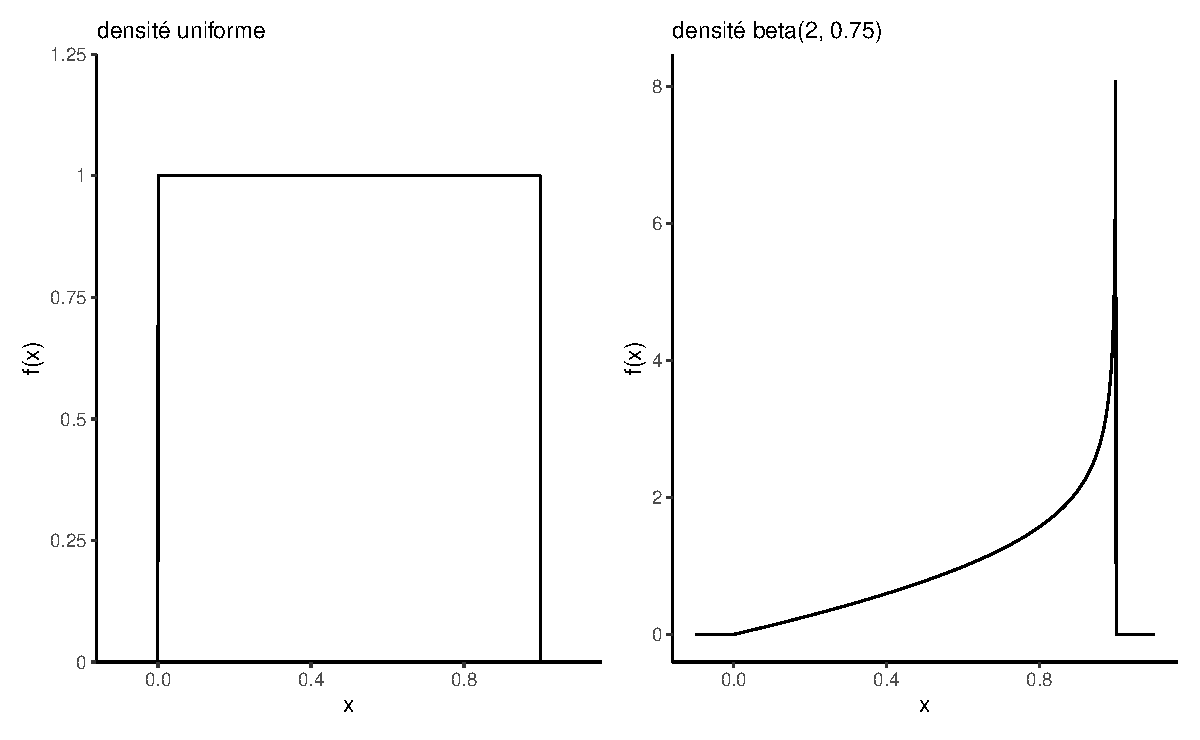
\includegraphics[width=0.85\textwidth,height=\textheight]{introduction_files/figure-pdf/fig-densite-beta-1.pdf}

}

\caption{\label{fig-densite-beta}Fonctions de densité de lois uniformes
et beta(2, 3/4) sur l'intervalle {[}0,1{]}.}

\end{figure}%

\end{definition}

\begin{definition}[Loi
exponentielle]\protect\hypertarget{def-loiexpo}{}\label{def-loiexpo}

La loi exponentielle figure de manière proéminente dans l'étude des
temps d'attente pour les phénomènes Poisson et en analyse de survie. Une
caractéristique clé de la loi est son absence de mémoire:
\(\Pr(Y \geq y + u \mid Y > u) = \Pr(Y > u)\) pour \(Y > 0\) et
\(y, u>0\).

La fonction de répartition de la loi exponentielle
\(Y \sim \mathsf{Exp}(\beta)\) où \(\beta>0\), est
\(F(x) = 1-\exp(-\beta x)\) et sa fonction de densité est
\(f(x) =\beta\exp(-\beta x)\) pour \(x >0\). La moyenne théorique de la
loi est \(\beta\).

\end{definition}

\begin{definition}[Loi
normale]\protect\hypertarget{def-loinormale}{}\label{def-loinormale}

De loin la plus continue des distributions, la loi normale intervient
dans le théorème central limite, qui dicte le comportement aléatoire de
la moyenne de grand échantillons. La fonction de densité est symmétrique
autour d'une moyenne \(\mu \in \mathbb{R}\), qui est une mesure de la
tendance centrale. L'autre paramètre, l'écart-type \(\sigma>0\), est un
paramètre d'échelle qui mesure la dispersion. La fonction de densité, en
forme de cloche, est symmétrique autour de \(\mu\), qui est aussi le
mode de la distribution.

\begin{figure}[ht!]

\centering{

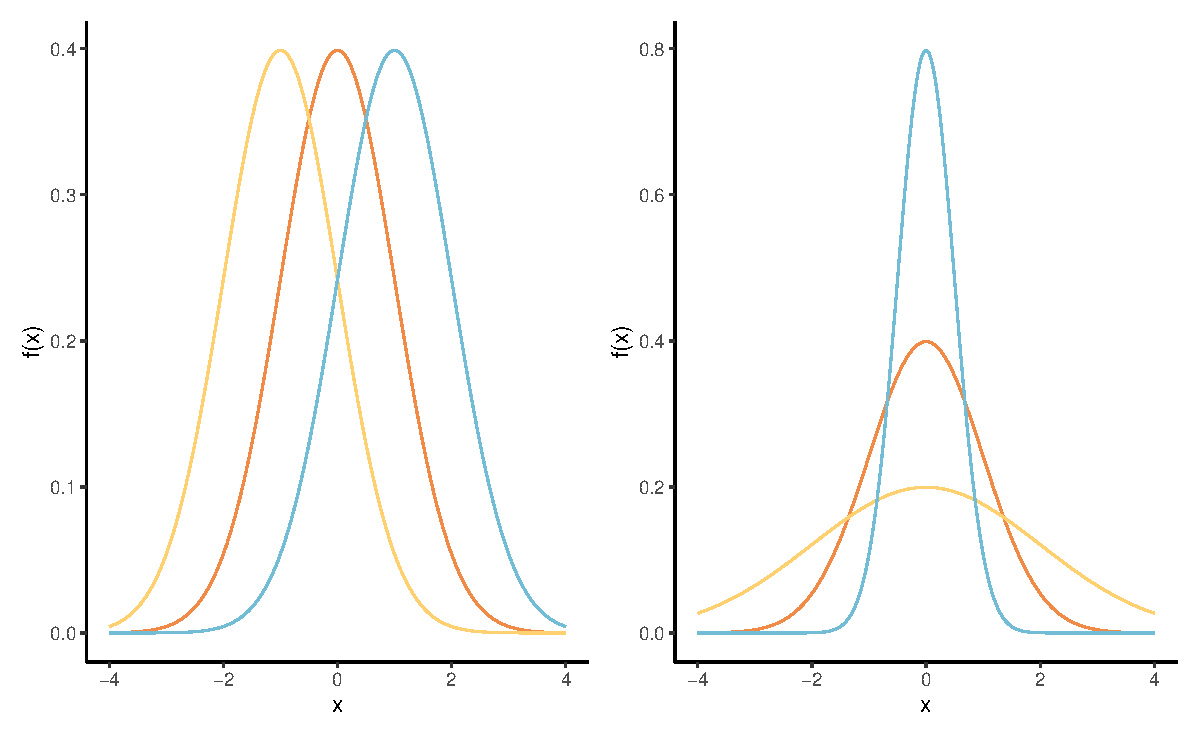
\includegraphics[width=0.85\textwidth,height=\textheight]{introduction_files/figure-pdf/fig-normal-loc-echelle-1.pdf}

}

\caption{\label{fig-normal-loc-echelle}Densités de loi normales avec des
paramètres de moyenne différents (gauche) et des paramètres d'échelle
différents (droite).}

\end{figure}%

La loi normale est une famille de localisation échelle: si
\(Y \sim \mathsf{normale}(\mu, \sigma^2)\), alors
\(Z = (Y-\mu)/\sigma \sim \mathsf{normale}(0,1)\). La variable
standardisée est appelée cote Z. Inversement, si
\(Z \sim \mathsf{normale}(0,1)\), alors
\(Y = \mu + \sigma Z \sim \mathsf{normale}(\mu, \sigma^2)\).

\end{definition}

Les trois lois suivantes ne sont pas couvertes dans les cours
d'introduction, mais elles interviennent régulièrement dans les cours de
mathématique statistique et serviront d'étalon de mesure pour déterminer
si les statistiques de test sont extrêmes sous l'hypothèse nulle.

\begin{definition}[Loi
khi-deux]\protect\hypertarget{def-loikhideux}{}\label{def-loikhideux}

La loi de khi-deux avec \(\nu>0\) degrés de liberté, dénotée
\(\chi^2_{\nu}\) joue un rôle important en statistique car elle est la
loi nulle asymptotique de nombreuses statistiques de test usuelles. Sa
densité est \begin{align*}
f(x; \nu) = \frac{1}{2^{\nu/2}\Gamma(\nu/2)}x^{\nu/2-1}\exp(-x/2),\qquad x >0.
\end{align*} Elle est obtenue en prenant la somme de variables normales
centrées et réduites au carré: si
\(Z_i \stackrel{\mathrm{iid}}{\sim}\mathsf{normale}(0,1)\) pour
\(i=1, \ldots, k\), alors \(\sum_{i=1}^k Z_i^2 \sim \chi^2_k\).
L'espérance de la loi \(\chi^2_k\) est \(k\).

\end{definition}

\begin{definition}[Loi
Student-\(t\)]\protect\hypertarget{def-loistudent}{}\label{def-loistudent}

La loi Student-\(t\) avec \(\nu>0\) degrés de liberté est une famille de
localisation et d'échelle de densité symmétrique. On la dénote
\(\mathsf{Student}(\nu)\) dans le cas centré réduit. Ses ailes sont plus
lourdes que la loi normale et son \(k\)e moment existe uniquement si
\(\nu > k\). Ainsi, la variance n'existe que si \(\nu>2\). Si
\(\nu \to \infty\), on recouvre une loi limite Gaussienne standard.

Son nom provient d'un article de William Gosset sous le pseudonyme
Student (\citeproc{ref-Student:1908}{Gosset 1908}). La statistique
\(T\), pour des données Gaussiennes, suit une loi Student avec \(k\)
degrés de liberté, puisque la moyenne est Gaussienne et la variance
empirique, adéquatement repondérée, suit une loi khi-deux avec \(k\)
degrés de liberté.

\begin{figure}[ht!]

{\centering 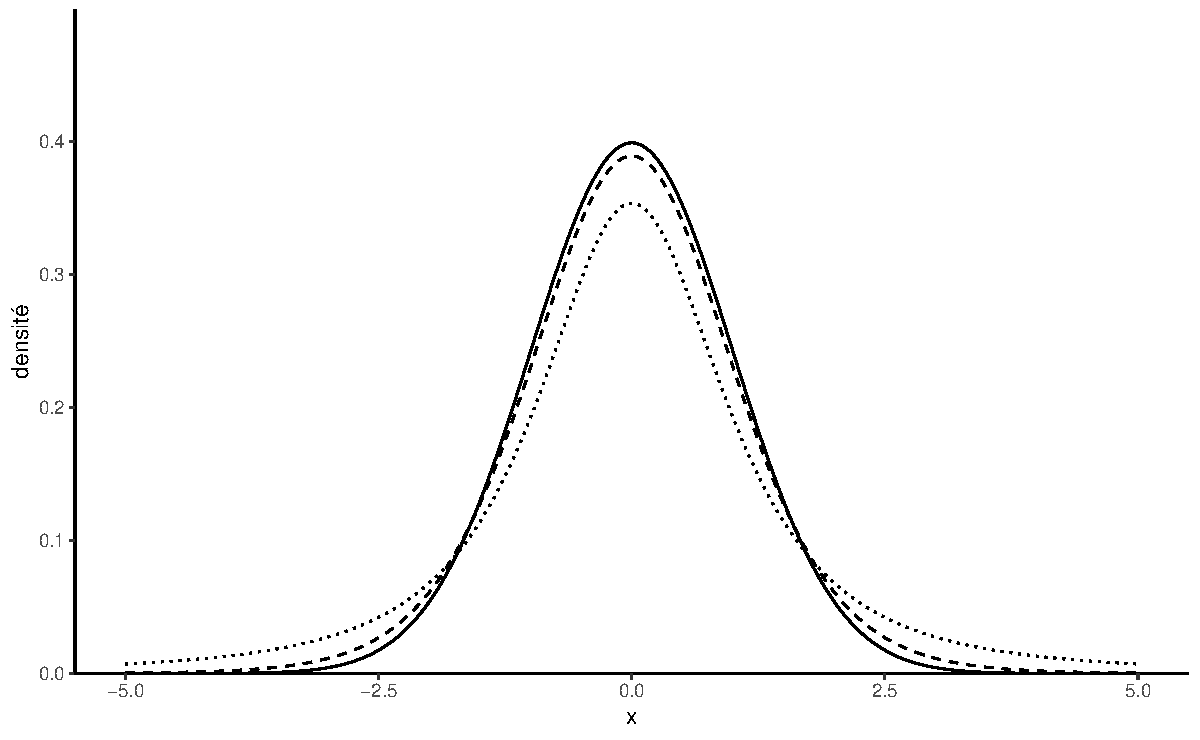
\includegraphics[width=0.5\textwidth,height=\textheight]{introduction_files/figure-pdf/unnamed-chunk-6-1.pdf}

}

\caption{Comparaison de la densité Student-\(t\) versus normale pour
différents degrés de liberté avec \(\nu=2\) (pointillé), \(\nu=10\)
(traitillé) et la loi normale (\(\nu = \infty)\).}

\end{figure}%

\end{definition}

\begin{definition}[Loi de
Fisher]\protect\hypertarget{def-loiF}{}\label{def-loiF}

Une généralisation de la loi Student-\(t\) est obtenue pour le
comportement en grand échantillon de statistiques de test pour la
comparaison de plusieurs moyennes (analyse de variance) sous un postulat
de normalité des observations.

La loi \(F\), dite de Fisher et dénotée
\(\mathsf{Fisher}(\nu_1, \nu_2)\), est obtenue en divisant deux
variables khi-deux indépendantes de degrés de liberté \(\nu_1\) et
\(\nu_2\). Spécifiquement, si \(Y_1 \sim \chi^2_{\nu_1}\) et
\(Y_2 \sim \chi^2_{\nu_2}\), alors \begin{align*}
F = \frac{Y_1/\nu_1}{Y_2/\nu_2} \sim \mathsf{Fisher}(\nu_1, \nu_2)
\end{align*}

La loi de Fisher tend vers une loi \(\chi^2\) quand
\(\nu_2 \to \infty\).

\end{definition}

\subsection{Graphiques}\label{graphiques}

Le principal type de graphique pour représenter la distribution d'une
variable catégorielle est le diagramme en bâtons, dans lequel la
fréquence de chaque catégorie est présentée sur l'axe des ordonnées
(\(y\)) en fonction de la modalité, sur l'axe des abscisses (\(x\)), et
ordonnées pour des variables ordinales. Cette représentation est en tout
point supérieur au
\href{http://www.perceptualedge.com/articles/08-21-07.pdf}{diagramme en
camembert}, une engeance répandu qui devrait être honnie (notamment
parce que l'humain juge mal les différences d'aires, qu'une simple
rotation change la perception du graphique et qu'il est difficile de
mesurer les proportions) --- ce n'est pas de la tarte!

\begin{figure}[ht!]

\centering{

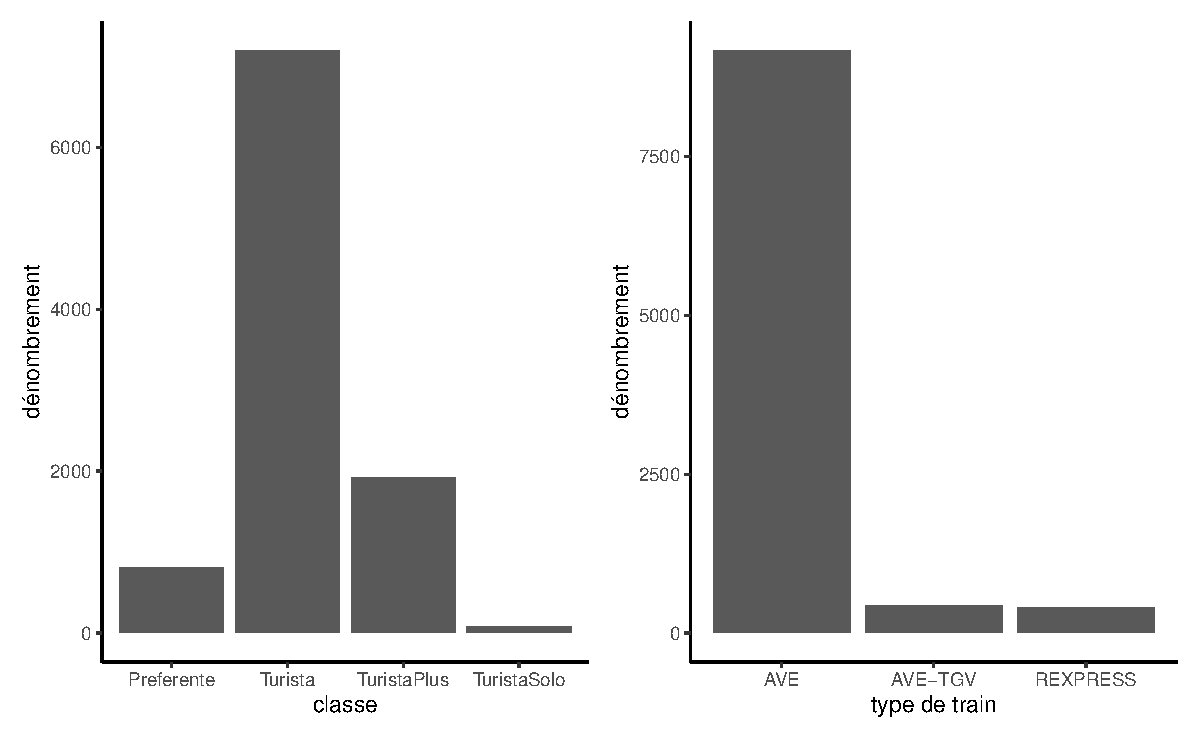
\includegraphics[width=0.85\textwidth,height=\textheight]{introduction_files/figure-pdf/fig-barplotrenfe-1.pdf}

}

\caption{\label{fig-barplotrenfe}Diagramme en bâtons pour la classe des
billets de trains du jeu de données Renfe.}

\end{figure}%

Puisque les variables continues peuvent prendre autant de valeurs
distinctes qu'il y a d'observations, on ne peut simplement compter le
nombre d'occurrence par valeur unique. On regroupera plutôt dans un
certain nombre d'intervalle, en discrétisant l'ensemble des valeurs en
classes pour obtenir un histogramme. Le nombre de classes dépendra du
nombre d'observations si on veut que l'estimation ne soit pas impactée
par le faible nombre d'observations par classe: règle générale, le
nombre de classes ne devrait pas dépasser \(\sqrt{n}\), où \(n\) est le
nombre d'observations de l'échantillon. On obtiendra la fréquence de
chaque classe, mais si on normalise l'histogramme (de façon à ce que
l'aire sous les bandes verticales égale un), on obtient une
approximation discrète de la fonction de densité. Faire varier le nombre
de classes permet parfois de faire apparaître des caractéristiques de la
variable (notamment la multimodalité, l'asymmétrie et les arrondis).

Puisque qu'on groupe les observations en classe pour tracer
l'histogramme, il est difficile de voir l'étendue des valeurs que prenne
la variable: on peut rajouter des traits sous l'histogramme pour
représenter les valeurs uniques prises par la variable, tandis que la
hauteur de l'histogramme nous renseigne sur leur fréquence relative.

\begin{figure}[ht!]

\centering{

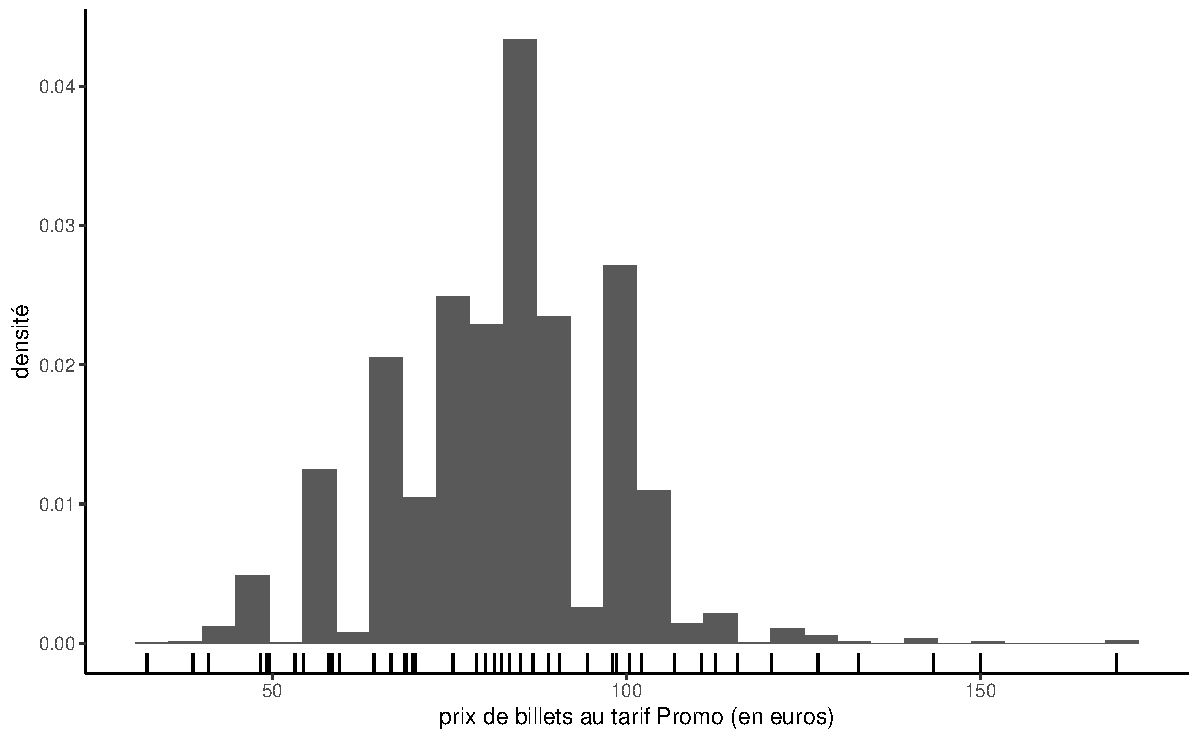
\includegraphics[width=0.85\textwidth,height=\textheight]{introduction_files/figure-pdf/fig-histrenfe-1.pdf}

}

\caption{\label{fig-histrenfe}Histogramme du prix des billets au tarif
Promo de trains du jeu de données Renfe}

\end{figure}%

\begin{definition}[Boîte à
moustaches]\protect\hypertarget{def-boxplot}{}\label{def-boxplot}

Elle représente graphiquement cinq statistiques descriptives.

\begin{itemize}
\tightlist
\item
  La boîte donne les 1e, 2e et 3e quartiles \(q_1, q_2, q_3\). Il y a
  donc 50\% des observations sont au-dessus/en-dessous de la médiane
  \(q_2\) qui sépare en deux la boîte.
\item
  La longueur des moustaches est moins de \(1.5\) fois l'écart
  interquartile \(q_3-q_1\) (tracée entre 3e quartile et le dernier
  point plus petit que \(q_3+1.5(q_3-q_1)\), etc.)
\item
  Les observations au-delà des moustaches sont encerclées. Notez que
  plus le nombre d'observations est élevé, plus le nombres de valeurs
  aberrantes augmente. C'est un défaut de la boîte à moustache, qui a
  été conçue pour des jeux de données qui passeraient pour petits selon
  les standards actuels.
\end{itemize}

\begin{figure}[ht!]

{\centering 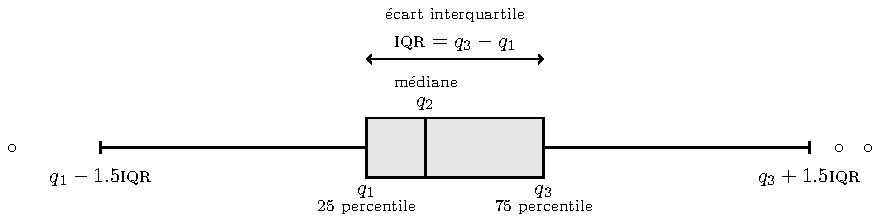
\includegraphics[width=0.85\textwidth,height=\textheight]{images/01-intro-boiteamoustache.pdf}

}

\caption{Boîte à moustache.}

\end{figure}%

\end{definition}

On peut représenter la distribution d'une variable réponse continue en
fonction d'une variable catégorielle en traçant une boîte à moustaches
pour chaque catégorie et en les disposant côte-à-côte. Une troisième
variable catégorielle peut être ajoutée par le biais de couleurs, comme
dans la Figure~\ref{fig-histboxplot}.

\begin{figure}[ht!]

\centering{

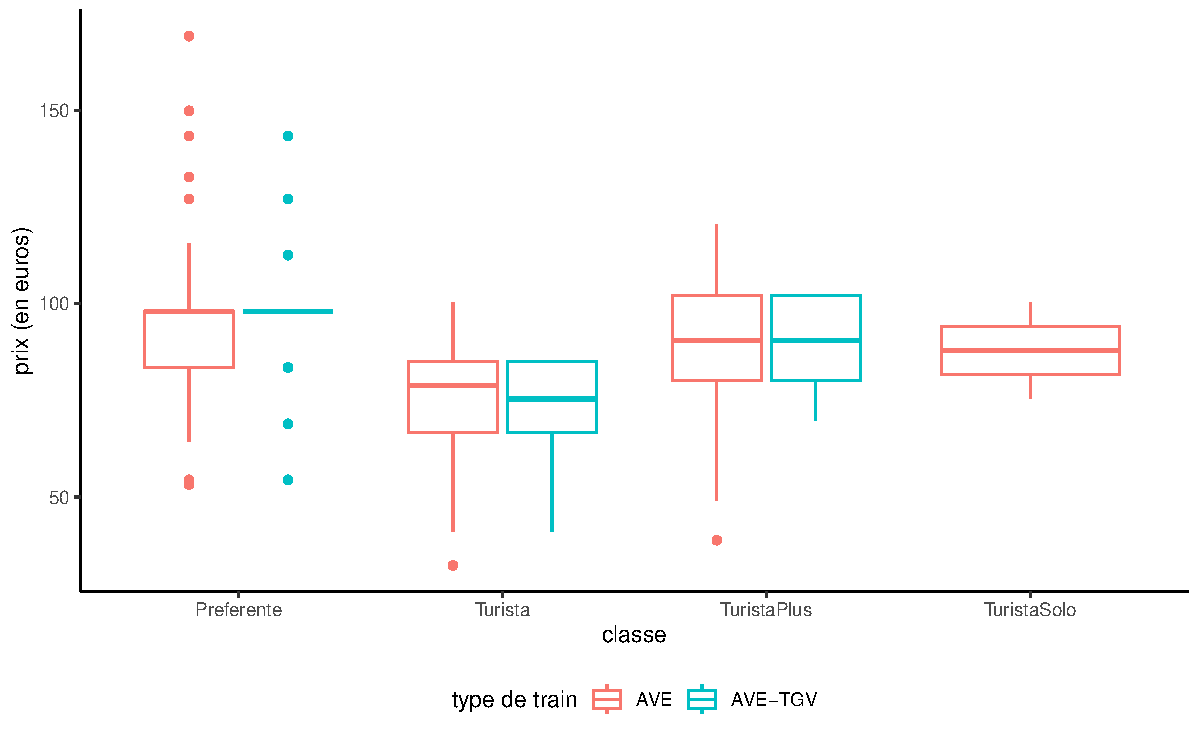
\includegraphics[width=0.85\textwidth,height=\textheight]{introduction_files/figure-pdf/fig-histboxplot-1.pdf}

}

\caption{\label{fig-histboxplot}Boîte à moustaches du prix des billets
au tarif Promo en fonction de la classe pour le jeu de données Renfe.}

\end{figure}%

Si on veut représenter la covariabilité de deux variables continues, on
utilise un nuage de points où chaque variable est représentée sur un axe
et chaque observation donne la coordonnée des points. Si la
représentation graphique est dominée par quelques valeurs très grandes,
une transformation des données peut être utile: vous verrez souvent des
données positives à l'échelle logarithmique.

\begin{definition}[Diagrammes
quantiles-quantiles]\protect\hypertarget{def-diagramme-qq}{}\label{def-diagramme-qq}

Si on ajuste un modèle à des données, il convient de vérifier la qualité
de l'ajustement et l'adéquation du modèle, par exemple graphiquement. Le
diagramme quantile-quantile sert à vérifier l'adéquation du modèle et
découle du constat suivant: si \(Y\) est une variable aléatoire continue
et \(F\) sa fonction de répartition, alors l'application
\(F(Y) \sim \mathsf{Unif}(0,1)\). De la même façon, appliquer la
fonction quantile à une variable uniforme permet de simuler de la loi
\(F\), et donc \(F^{-1}(U)\).

Les paramètres de la loi \(F\) sont inconnus, mais on peut obtenir un
estimateur \(\widehat{F}\) et appliquer la transformation inverse pour
obtenir une variable approximativement uniforme. Un diagramme
quantile-quantile représente les données en fonction des moments des
statistiques d'ordre transformées

\begin{itemize}
\tightlist
\item
  sur l'axe des abscisses, les quantiles théoriques
  \(\widehat{F}^{-1}\{\mathrm{rang}(Y_i)/(n+1)\}\)
\item
  sur l'axe des ordonnées, les quantiles empiriques \(Y_i\)
\end{itemize}

Si le modèle est adéquat, les valeurs ordonnées devraient suivre une
droite de pente unitaire qui passe par l'origine. Le diagramme
probabilité-probabilité représente plutôt les données à l'échelle
uniforme \(\{\mathrm{rang}(Y_i)/(n+1), \widehat{F}(Y_i)\}\).

\end{definition}

\begin{figure}[ht!]

\centering{

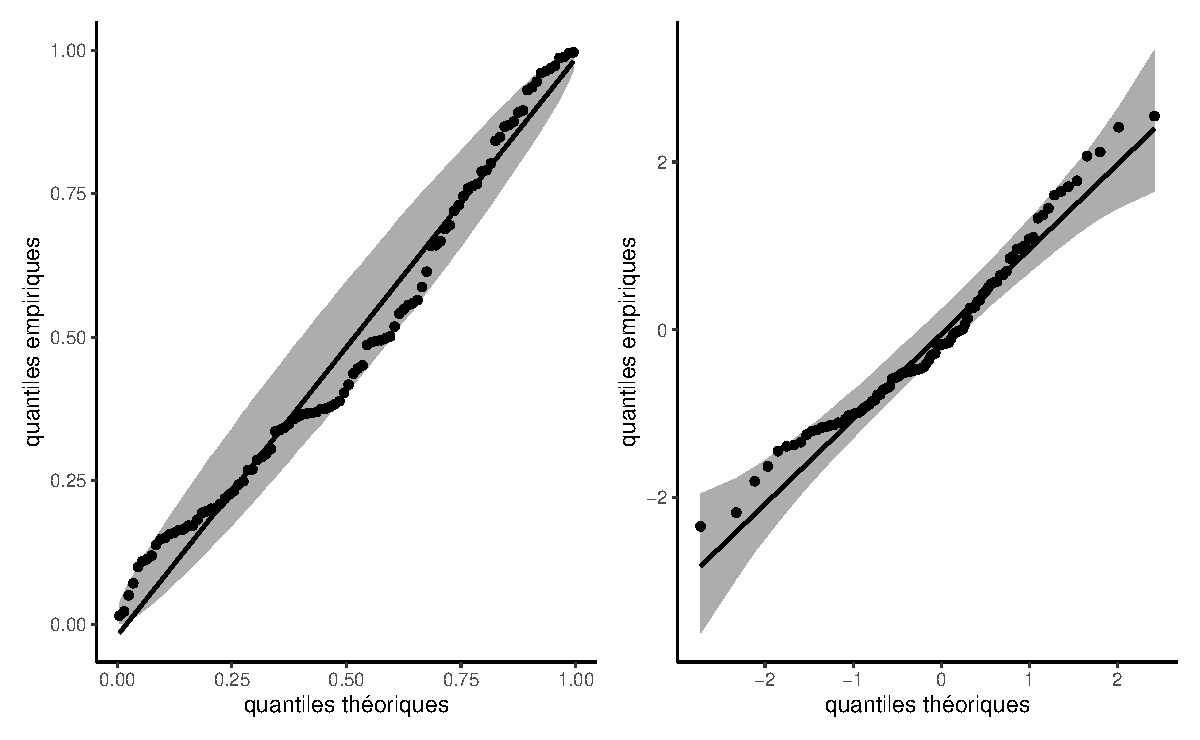
\includegraphics[width=0.85\textwidth,height=\textheight]{introduction_files/figure-pdf/fig-diagrammeqq2-1.pdf}

}

\caption{\label{fig-diagrammeqq2}Diagramme probabilité-probabilité
(gauche) et quantile-quantile normal (droite)}

\end{figure}%

Même si on connaissait exactement la loi aléatoire des données, la
variabilité intrinsèque à l'échantillon fait en sorte que des déviations
qui semblent significatives et anormales à l'oeil de l'analyste sont en
fait compatibles avec le modèle: un simple estimé ponctuel sans mesure
d'incertitude ne permet donc pas facilement de voir ce qui est plausible
ou pas. On va donc idéalement ajouter un intervalle de confiance
(approximatif) ponctuel ou conjoint au diagramme.

Pour obtenir l'intervalle de confiance approximatif, la méthode la plus
simple est par simulation (autoamorçage paramétrique), en répétant \(B\)
fois les étapes suivantes

\begin{enumerate}
\def\labelenumi{\arabic{enumi}.}
\tightlist
\item
  simuler un échantillon \(\{Y^{(b)}_{i}\} (i=1,\ldots, n)\) du modèle
  \(\widehat{F}\)
\item
  estimer les paramètres du modèle \(F\) pour obtenir
  \(\widehat{F}_{(b)}\)
\item
  calculer et stocker les positions
  \(\widehat{F}^{-1}_{(b)}\{i/(n+1)\}\).
\end{enumerate}

Le résultat de cette opération sera une matrice \(n \times B\) de
données simulées; on obtient un intervalle de confiance symmétrique en
conservant le quantile \(\alpha/2\) et \(1-\alpha/2\) de chaque ligne.
Le nombre de simulation \(B\) devrait être large (typiquement 999 ou
davantage) et être choisi de manière à ce que \(B/\alpha\) soit un
entier.

Pour l'intervalle de confiance ponctuel, chaque valeur représente une
statistique et donc individuellement, la probabilité qu'une statistique
d'ordre sorte de l'intervalle de confiance est \(\alpha\). En revanche,
les statistiques d'ordres ne sont pas indépendantes et sont qui est plus
ordonnées, ce qui fait qu'un point hors de l'intervalle risque de n'être
pas isolé. Les intervalles présentés dans la
Figure~\ref{fig-diagrammeqq2} sont donc ponctuels. La variabilité des
statistiques d'ordre uniformes est plus grande autour de 1/2, mais
celles des variables transformées dépend de \(F\).

\subsection{Loi des grands nombres}\label{loi-grands-nombres}

Un estimateur est dit \textbf{convergent} si la valeur obtenue à mesure
que la taille de l'échantillon augmente s'approche de la vraie valeur
que l'on cherche à estimer. Mathématiquement parlant, un estimateur est
dit convergent s'il converge en probabilité, ou
\(\hat{\theta} \stackrel{\mathsf{Pr}}{\to} \theta\): en langage commun,
la probabilité que la différence entre \(\hat{\theta}\) et \(\theta\)
diffèrent est négligeable quand \(n\) est grand.

La condition \emph{a minima} pour le choix d'un estimateur est donc la
convergence: plus on récolte d'information, plus notre estimateur
devrait s'approcher de la valeur qu'on tente d'estimer.

La loi des grands nombres établit que la moyenne empirique de \(n\)
observations indépendantes de même espérance, \(\overline{Y}_n\), tend
vers l'espérance commune des variables \(\mu\), où
\(\overline{Y}_n \rightarrow \mu\). En gros, ce résultat nous dit que
l'on réussit à approximer de mieux en mieux la quantité d'intérêt quand
la taille de l'échantillon (et donc la quantité d'information disponible
sur le paramètre) augmente. La loi des grands nombres est très utile
dans les expériences Monte Carlo: on peut ainsi approximer par
simulation la moyenne d'une fonction \(g(x)\) de variables aléatoires en
simulant de façon répétée des variables \(Y\) indépendantes et
identiquement distribuées et en prenant la moyenne empirique
\(n^{-1} \sum_{i=1}^n g(Y_i)\).

Si la loi des grands nombres nous renseigne sur le comportement limite
ponctuel, il ne nous donne aucune information sur la variabilité de
notre estimé de la moyenne et la vitesse à laquelle on s'approche de la
vraie valeur du paramètre.

\subsection{Théorème central limite}\label{TCL}

Le théorème central limite dit que, pour un échantillon aléatoire de
taille \(n\) dont les observations sont indépendantes et tirées d'une
loi quelconque d'espérance \(\mu\) et de variance finie \(\sigma^2\),
alors la moyenne empirique tend non seulement vers \(\mu\), mais à une
vitesse précise:

\begin{itemize}
\tightlist
\item
  l'estimateur \(\overline{Y}\) sera centré autour de \(\mu\),
\item
  l'erreur-type sera de \(\sigma/\sqrt{n}\); le taux de convergence est
  donc de \(\sqrt{n}\). Ainsi, pour un échantillon de taille 100,
  l'erreur-type de la moyenne empirique sera 10 fois moindre que
  l'écart-type de la variable aléatoire sous-jacente.
\item
  la loi approximative de la moyenne \(\overline{Y}\) sera normale.
\end{itemize}

Mathématiquement, le théorème central limite dicte que
\(\sqrt{n}(\overline{Y}-\mu) \stackrel{\mathrm{d}}{\rightarrow} \mathsf{normale}(0, \sigma^2)\).
Si \(n\) est grand (typiquement supérieur à \(30\), mais cette règle
dépend de la loi sous-jacente de \(Y\)), alors
\(\overline{Y} \stackrel{\cdot}{\sim} \mathsf{normale}(\mu, \sigma^2/n)\).

Comment interpréter ce résultat? On considère comme exemple le temps de
trajet moyen de trains à haute vitesse AVE entre Madrid et Barcelone
opérés par la Renfe.

\begin{figure}[ht!]

\centering{

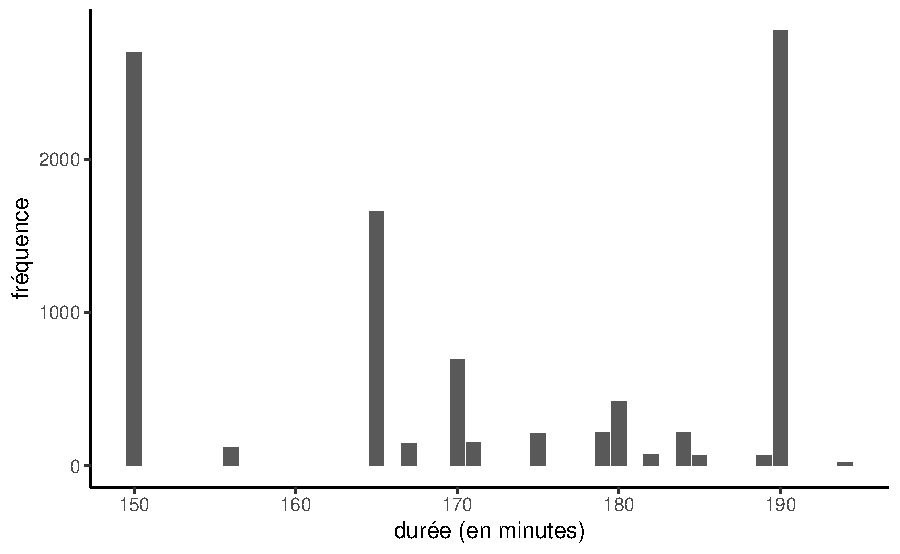
\includegraphics[width=0.85\textwidth,height=\textheight]{introduction_files/figure-pdf/fig-renfeclt-1.pdf}

}

\caption{\label{fig-renfeclt}Distribution empirique des temps de trajet
en trains à grande vitesse.}

\end{figure}%

Une analyse exploratoire indique que la durée du trajet de la base de
données est celle affichée sur le billet (et non le temps réel du
parcours). Ainsi, il n'y a ainsi que 15 valeurs possibles. Le temps
affiché moyen pour le parcours, estimé sur la base de 9603 observations,
est de 170 minutes et 41 secondes. La Figure~\ref{fig-renfeclt} montre
la distribution empirique des données.

Considérons maintenant des échantillons de taille \(n=10\). Dans notre
premier échantillon aléatoire, la durée moyenne affichée est 170.9
minutes, elle est de 164.5 minutes dans le deuxième, de 172.3 dans le
troisième, et ainsi de suite.

\begin{figure}[ht!]

\centering{

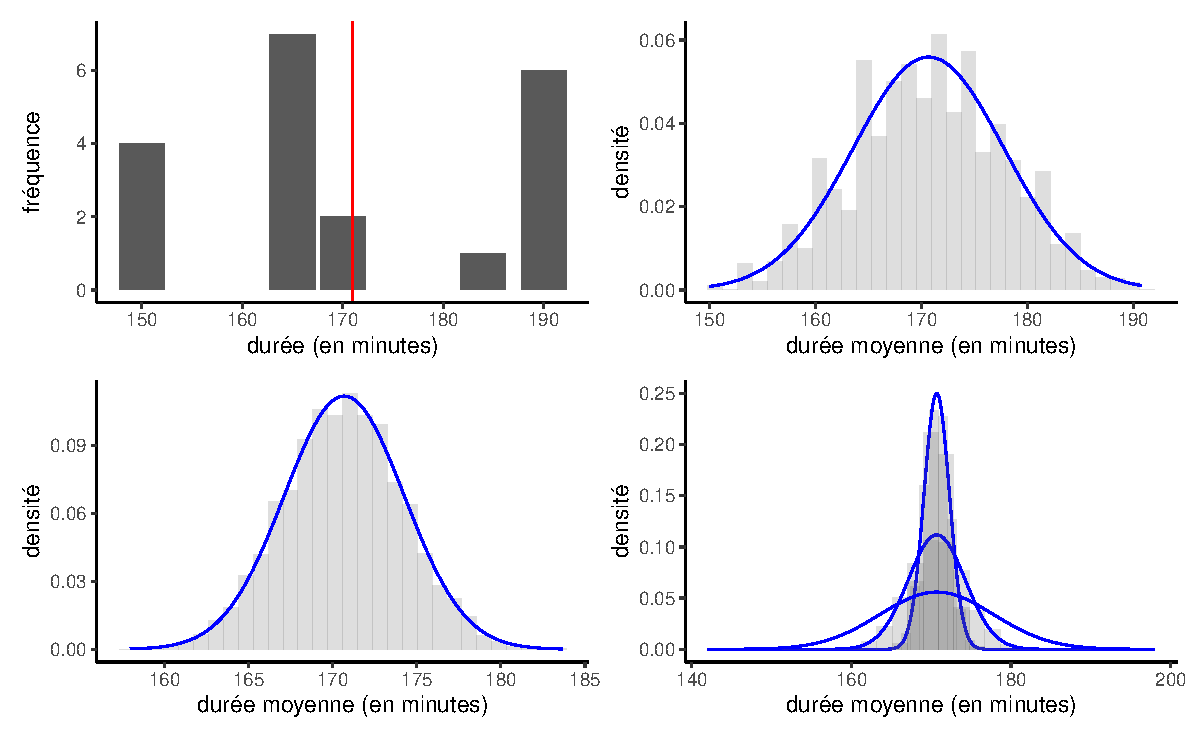
\includegraphics[width=0.9\textwidth,height=\textheight]{introduction_files/figure-pdf/fig-renfemeanCLT-1.pdf}

}

\caption{\label{fig-renfemeanCLT}Représentation graphique du théorème
central limite: échantillon aléatoire de 20 observations avec leur
moyenne empirique (trait vertical rouge) (en haut à gauche). Les trois
autres panneaux montrent les histogrammes des moyennes empiriques
d'échantillons répétés de taille 5 (en haut à droite), 20 (en bas à
gauche) et les histogrammes pour \(n=5, 20, 100\) (en bas à droite) avec
courbe de densité de l'approximation normale fournie par le théorème
central limite.}

\end{figure}%

Supposons qu'on tire \(B=1000\) échantillons différents, chacun de
taille \(n=5\), de notre ensemble, et qu'on calcule la moyenne de chacun
d'entre eux. Le graphique supérieur droit de la
Figure~\ref{fig-renfemeanCLT} montre un de ces 1000 échantillons
aléatoire de taille \(n=20\) tiré de notre base de données. Les autres
graphiques de la Figure~\ref{fig-renfemeanCLT} illustrent l'effet de
l'augmentation de la taille de l'échantillon: si l'approximation normale
est approximative avec \(n=5\), la distribution des moyennes est
virtuellement identique à partir de \(n=20\). Plus la moyenne est
calculée à partir d'un grand échantillon (c'est-à-dire, plus \(n\)
augmente), plus la qualité de l'approximation normale est meilleure et
plus la courbe se concentre autour de la vraie moyenne; malgré le fait
que nos données sont discrètes, la distribution des moyennes est
approximativement normale.

On a considéré une seule loi aléatoire inspirée de l'exemple, mais vous
pouvez vous amuser à regarder l'effet de la distribution sous-jacent et
de la taille de l'échantillon nécessaire pour que l'effet du théorème
central limite prenne effet: il suffit pour cela de simulant des
observations d'une loi quelconque de variance finie, en utilisant par
exemple cette
\href{http://195.134.76.37/applets/AppletCentralLimit/Appl_CentralLimit2.html}{applette}.

Les statistiques de test qui découlent d'une moyenne centrée-réduite (ou
d'une quantité équivalente pour laquelle un théorème central limite
s'applique) ont souvent une loi nulle standard normale, du moins
asymptotiquement (quand \(n\) est grand, typiquement \(n>30\) est
suffisant). C'est ce qui garantie la validité de notre inférence!

\bookmarksetup{startatroot}

\chapter{Inférence statistique}\label{inference}

\section{Tests d'hypothèse}\label{tests}

Un test d'hypothèse statistique est une façon d'évaluer la preuve
statistique provenant d'un échantillon afin de faire une décision quant
à la population sous-jacente. Les étapes principales sont:

\begin{itemize}
\tightlist
\item
  définir les paramètres du modèle,
\item
  formuler les hypothèses alternative et nulle,
\item
  choisir et calculer la statistique de test,
\item
  déterminer son comportement sous \(\mathscr{H}_0\) (loi nulle),
\item
  calculer la valeur-\emph{p},
\item
  conclure dans le contexte du problème (rejeter ou ne pas rejeter
  \(\mathscr{H}_0\)).
\end{itemize}

Mon approche privilégiée pour présenter les tests d'hypothèse est de
faire un parallèle avec un procès pour meurtre où vous êtes nommé juré.

\begin{itemize}
\tightlist
\item
  Le juge vous demande de choisir entre deux hypothèses mutuellement
  exclusives, coupable ou non-coupable, sur la base des preuves
  présentées.
\item
  Votre postulat de départ repose sur la présomption d'innocence: vous
  condamnerez uniquement le suspect si la preuve est accablante. Cela
  permet d'éviter les erreurs judiciaires. L'hypothèse nulle
  \(\mathscr{H}_0\) est donc \emph{non-coupable}, et l'hypothèse
  alternative \(\mathscr{H}_a\) est coupable. En cas de doute
  raisonnable, vous émettrez un verdict de non-culpabilité.
\item
  La choix de la statistique de test représente la preuve. Plus la
  preuve est accablante, plus grande est la chance d'un verdict de
  culpabilité --- le procureur a donc tout intérêt à bien choisir les
  faits présentés en cour. Le choix de la statistique devrait donc
  idéalement maximiser la preuve pour appuyer le postulat de culpabilité
  le mieux possible (ce choix reflète la \textbf{puissance} du test).
\item
  En qualité de juré, vous analysez la preuve à partir de la
  jurisprudence et de l'avis d'expert pour vous assurer que les faits ne
  relèvent pas du hasard. Pour le test d'hypothèse, ce rôle est tenu par
  la loi sous \(\mathscr{H}_0\): si la personne était innocente, est-ce
  que les preuves présentées tiendraient la route? des traces d'ADN
  auront davantage de poids que des ouï-dire (la pièce de théâtre
  \emph{Douze hommes en colère} de Reginald Rose présente un bel exemple
  de procès où un des juré émet un doute raisonnable et convainc un à un
  les autres membres du jury de prononcer un verdict de
  non-culpabilité).
\item
  Vous émettez un verdict, à savoir une décision binaire, où l'accusé
  est déclaré soit non-coupable, soit coupable. Si vous avez une
  valeur-\emph{p}, disons \(P\), pour votre statistique de test et que
  vous effectuez ce dernier à niveau \(\alpha\), la règle de décision
  revient à rejeter \(\mathscr{H}_0\) si \(P < \alpha\).
\end{itemize}

On s'attarde davantage sur ces définitions heuristiques et le
vocabulaire employé pour parler de tests d'hypothèse. Le matériel de la
section suivante a été préparé par Juliana Schulz.

\section{Hypothèse}\label{hypothuxe8se}

Dans les test statistique il y a toujours deux hypothèse: l'hypothèse
nulle (\(\mathscr{H}_{0}\)) et l'hypothèse alternative
(\(\mathscr{H}_a\)). Habituellement, l'hypothèse nulle est le « statu
quo » et l'alternative est l'hypothèse que l'on cherche à démontrer. On
se fait l'avocat du Diable en défendant l'hypothèse nulle et en
analysant toutes les preuves sous l'angle: « est-ce que les données
entrent en contradiction avec \(\mathscr{H}_0\)? ». Un test d'hypothèse
statistique nous permet de décider si nos données nous fournissent assez
de preuves pour rejeter \(\mathscr{H}_0\) en faveur de
\(\mathscr{H}_a\), selon un risque d'erreur spécifié.

Généralement, les tests d'hypothèses sont exprimés en fonction de
paramètres (de valeurs inconnues) du modèle sous-jacent, par ex.
\(\theta\). Un test d'hypothèse bilatéral concernant un paramètre
scalaire \(\theta\) s'exprimerait la forme suivante: \begin{align*}
\mathscr{H}_0: \theta=\theta_0 \qquad \text{versus} \qquad \mathscr{H}_a:\theta \neq \theta_0.
\end{align*} Ces hypothèses permettent de tester si \(\theta\) est égal
à une valeur numérique précise \(\theta_0\).

Par exemple, pour un test bilatéral concernant le paramètre d'un modèle
de régression \(\beta_j\) associé à une variable explicative d'intérêt
\(\mathrm{X}_j\), les hypothèses sont \begin{align*}
\mathscr{H}_0: \beta_j=\beta_j^0 \qquad \text{versus} \qquad \mathscr{H}_a:\beta_j \neq \beta_j^0,
\end{align*} où \(\beta_j^0\) est une valeur précise qui est reliée à la
question de recherche. Par exemple, si \(\beta_j^0=0\) la question de
recherche sous-jacente est: est-ce que la covariable \(\mathrm{X}_j\)
impacte la variable réponse d'intérêt \(Y\) une fois l'effet des autres
variables pris en compte?

Remarque: il est possible d'imposer une direction dans les tests en
considérant une hypothèse alternative de la forme
\(\mathscr{H}_a: \theta > \theta_0\) ou
\(\mathscr{H}_a: \theta < \theta_0\).

\section{Statistique de test}\label{statistique-de-test}

Une statistique de test \(T\) est un fonctionnel des données qui résume
l'information contenue dans les données pour \(\theta\). La forme de la
statistique de test est choisie de façon à ce que son comportement sous
\(\mathscr{H}_0\), c'est-à-dire l'ensemble des valeurs que prend \(T\)
si \(\mathscr{H}_0\) est vraie et leur probabilité relative, soit connu.
En effet, \(T\) est une variable aléatoire et sa valeur va changer selon
l'échantillon. La \textbf{loi nulle} de la statistique de test nous
permet de déterminer quelles valeurs de \(T\) sont plausibles si
\(\mathscr{H}_0\) est vraie. Plusieurs statistiques que l'on couvrira
dans ce cours sont des \textbf{statistiques de Wald}, de la forme
\begin{align*}
T = \frac{\widehat{\theta} - \theta_0}{\mathrm{se}(\widehat{\theta})}
\end{align*} où \(\widehat{\theta}\) est l'estimateur du paramètre
\(\theta\), \(\theta_0\) la valeur numérique postulée (par ex., zéro) et
\(\mathrm{se}(\widehat{\theta})\) est l'estimateur de l'écart-type de
\(\widehat{\theta}\).

Par exemple, pour une hypothèse sur la moyenne d'une population de la
forme \begin{align*}
\mathscr{H}_0: \mu=0, \qquad  \mathscr{H}_a:\mu \neq 0,
\end{align*} la statistique de test de Wald est \begin{align*}
T &= \frac{\overline{X}-0}{S_n/\sqrt{n}}
\end{align*} où \(\overline{X}\) est la moyenne de l'échantillon
\(X_1, \ldots, X_n\), \begin{align*}
\overline{X} &= \frac{1}{n} \sum_{i=1}^n X_i = \frac{X_1+ \cdots + X_n}{n}
\end{align*} et l'erreur-type de la moyenne \(\overline{X}\) est
\(S_n/\sqrt{n}\); l'écart-type \(S_n\) est un estimateur de \(\sigma\),
où \begin{align*}
S^2_n &= \frac{1}{n-1} \sum_{i=1}^n (X_i-\overline{X})^2.
\end{align*}

Il convient de faire la différence entre procédures/formules et valeurs
numériques. Un \textbf{estimateur} est une règle ou une formule utilisée
pour calculer l'estimation d'un paramètre ou quantité d'intérêt selon
des données observées. Par exemple, la moyenne d'échantillon
\(\overline{X}\) est un estimateur de la moyenne dans la population
\(\mu\). Une fois qu'on a des données observées, on peut calculer un
estimé de la moyenne empirique \(\overline{x},\) c'est-à-dire, on
obtient une valeur numérique. Autrement dit,

\begin{itemize}
\tightlist
\item
  un estimateur est une fonction de variables aléatoires et donc c'est
  aussi une variable aléatoire car sa valeur fluctue d'un échantillon à
  l'autre.
\item
  l'estimé est la valeur numérique calculée sur un échantillon donné.
\end{itemize}

\section{\texorpdfstring{Loi nulle et
valeur-\emph{p}}{Loi nulle et valeur-p}}\label{loi-nulle-et-valeur-p}

La \textbf{valeur-\emph{p}} nous permet de déterminer si la valeur
observée de la statistique de test \(T\) est plausible sous
\(\mathscr{H}_0\). Plus précisément, la valeur-\emph{p} est la
probabilité, si \(\mathscr{H}_0\) est vraie, que la statistique de test
soit égale or plus extrême à ce qu'on observe. Supposons qu'on a un
échantillon \(X_1, \ldots, X_n\) et qu'on observe une valeur de la
statistique de test de \(T=t\). Pour un test d'hypothèse bilatéral
\(\mathscr{H}_0:\theta=\theta_0\)
vs.~\(\mathscr{H}_a:\theta \neq \theta_0\), la valeur-\emph{p} est
\(\mathsf{Pr}_0(|T| \geq |t|)\). Si la distribution de \(T\) est
symétrique autour de zéro, la valeur-\emph{p} vaut \begin{align*}
p = 2 \times \mathsf{Pr}_0(T \geq |t|).
\end{align*}

Prenons l'exemple d'un test d'hypothèse bilatéral pour la moyenne au
population \(\mathscr{H}_0:\mu=0\) contre \(\mathscr{H}_a:\mu \neq 0\).
Si l'échantillon provient d'une (population de) loi normale
\(\mathsf{Norm}(\mu, \sigma^2)\), on peut démontrer que, si
\(\mathscr{H}_0\) est vraie et donc \(\mu=0\)), la statistique de test
\begin{align*}
T = \frac{\overline{X}}{S/\sqrt{n}}
\end{align*} suit une loi de Student-\(t\) avec \(n-1\) degrés de
liberté, dénotée \(\mathsf{St}_{n-1}\). À partir de cette loi nulle, on
peut calculer la valeur-\emph{p} (ou bien à partir d'une table ou d'un
logiciel statistique). Puisque la distribution Student-\(t\) est
symétrique autour de \(0\), on peut calculer la valeur-\emph{p} comme
\(P = 2\times\mathsf{Pr}(T > |t|)\), où \(T \sim \mathsf{St}_{n-1}\).

\section{Conclusion}\label{conclusion}

La valeur-\emph{p} nous permet de faire une décision quant aux
hypothèses du test. Si \(\mathscr{H}_0\) est vraie, la valeur-\emph{p}
suit une loi uniforme. \href{https://xkcd.com/1478/}{Si la
valeur-\emph{p} est petite}, ça veut dire que le fait d'observer une
statistique de test égal ou encore plus extrême que \(T=t\) est peu
probable, et donc nous aurons tendance de croire que \(\mathscr{H}_0\)
n'est pas vraie. Il y a pourtant toujours un risque sous-jacent de
commettre un erreur quand on prend une décision. En statistique, il y a
\href{https://xkcd.com/2303/}{deux types d'erreurs}:

\begin{itemize}
\tightlist
\item
  erreur de type I: on rejette \(\mathscr{H}_0\) alors que
  \(\mathscr{H}_0\) est vraie
\item
  erreur de type II: on ne rejette pas \(\mathscr{H}_0\) alors que
  \(\mathscr{H}_0\) est fausse
\end{itemize}

Ces deux erreurs ne sont pas égales: on cherche souvent à contrôler
l'erreur de type I (une erreur judiciaire, condamner un innocent). Pour
se prémunir face à ce risque, on fixe préalablement un niveau de
tolérance. Plus notre seuil de tolérance \(\alpha\) est grand, plus on
rejette souvent l'hypothèse nulle même si cette dernière est vraie. La
valeur de \(\alpha \in (0, 1)\) est la probabilité qu'on rejette
\(\mathscr{H}_0\) quand \(\mathscr{H}_0\) est en fait vraie.
\begin{align*}
\alpha = \mathsf{Pr}_0\left(\text{ rejeter } \mathscr{H}_0\right).
\end{align*} Comme chercheur, on choisit ce niveau \(\alpha\);
habituellement \(1\)\%, \(5\)\% ou \(10\)\%. La probabilité de commettre
une erreur de type I est \(\alpha\) seulement si le modèle nul postulé
pour \(\mathscr{H}_0\) est correctement spécifié (sic) et correspond au
modèle générateur des données.

Le choix du statu quo (typiquement \(\mathscr{H}_0\)) s'explique plus
facilement avec un exemple médical. Si vous voulez prouver qu'un nouveau
traitement est meilleur que l'actuel (ou l'absence de traitement), vous
devez démontrer hors de tout doute raisonnable que ce dernier ne cause
pas de torts aux patients et offre une nette amélioration (pensez à
Didier Raoult et ses allégations non-étayées voulant que
l'hydrochloroquine, un antipaludique, soit efficace face au virus de la
Covid19).

\begin{longtable}[]{@{}
  >{\raggedright\arraybackslash}p{(\columnwidth - 4\tabcolsep) * \real{0.3333}}
  >{\centering\arraybackslash}p{(\columnwidth - 4\tabcolsep) * \real{0.3333}}
  >{\centering\arraybackslash}p{(\columnwidth - 4\tabcolsep) * \real{0.3333}}@{}}
\toprule\noalign{}
\begin{minipage}[b]{\linewidth}\raggedright
\textbf{Décision} \textbackslash{} \textbf{vrai modèle}
\end{minipage} & \begin{minipage}[b]{\linewidth}\centering
\(\mathscr{H}_0\)
\end{minipage} & \begin{minipage}[b]{\linewidth}\centering
\(\mathscr{H}_a\)
\end{minipage} \\
\midrule\noalign{}
\endhead
\bottomrule\noalign{}
\endlastfoot
ne pas rejeter \(\mathscr{H}_0\) & \(\checkmark\) & erreur de type II \\
rejeter \(\mathscr{H}_0\) & erreur de type I & \(\checkmark\) \\
\end{longtable}

Pour prendre une décision, on doit comparer la valeur-\emph{p} \(P\)
avec le niveau du test \(\alpha\):

\begin{itemize}
\tightlist
\item
  si \(P < \alpha\) on rejette \(\mathscr{H}_0\),
\item
  si \(P \geq \alpha\) on ne rejette pas \(\mathscr{H}_0\).
\end{itemize}

Attention à ne pas confondre niveau du test (probabilité fixée au
préalable par l'expérimentateur) et la valeur-\emph{p} (qui dépend de
l'échantillon). Si vous faites un test à un niveau 5\% la probabilité de
faire une erreur de type I est de 5\% par définition, quelque soit la
valeur de la valeur-\emph{p}. La valeur-\emph{p} s'interprète comme la
probabilité d'obtenir une valeur de la statistique de test égale ou même
plus grande que celle qu'on a observée dans l'échantillon, si
\(\mathscr{H}_0\) est vraie.

\section{Puissance statistique}\label{puissance-statistique}

Le but du test d'hypothèse est de prouver (hors de tout doute
raisonnable) qu'une différence ou un effet est significatif:: par
exemple, si une nouvelle configuration d'un site web (hypothèse
alternative) permet d'augmenter les ventes par rapport au statu quo.
Notre capacité à détecter cette amélioration dépend de la puissance du
test: plus cette dernière est élevée, plus grande est notre capacité à
rejeter \(\mathscr{H}_0\) quand ce dernier est faux. Quand on ne rejette
pas \(\mathscr{H}_0\) et que \(\mathscr{H}_a\) est en fait vraie, on
commet une erreur de type II: cette dernière survient avec probabilité
\(1-\gamma\). La \textbf{puissance statistique} d'un test est la
probabilité que le test rejette \(\mathscr{H}_0\) alors que
\(\mathscr{H}_0\) est fausse, soit \begin{align*}
\gamma = \mathsf{Pr}_a(\text{rejeter } \mathscr{H}_0)
\end{align*} Selon le choix de l'alternative, il est plus ou moins
facile de rejeter l'hypothèse nulle en faveur de l'alternative.

\begin{figure}[ht!]

\centering{

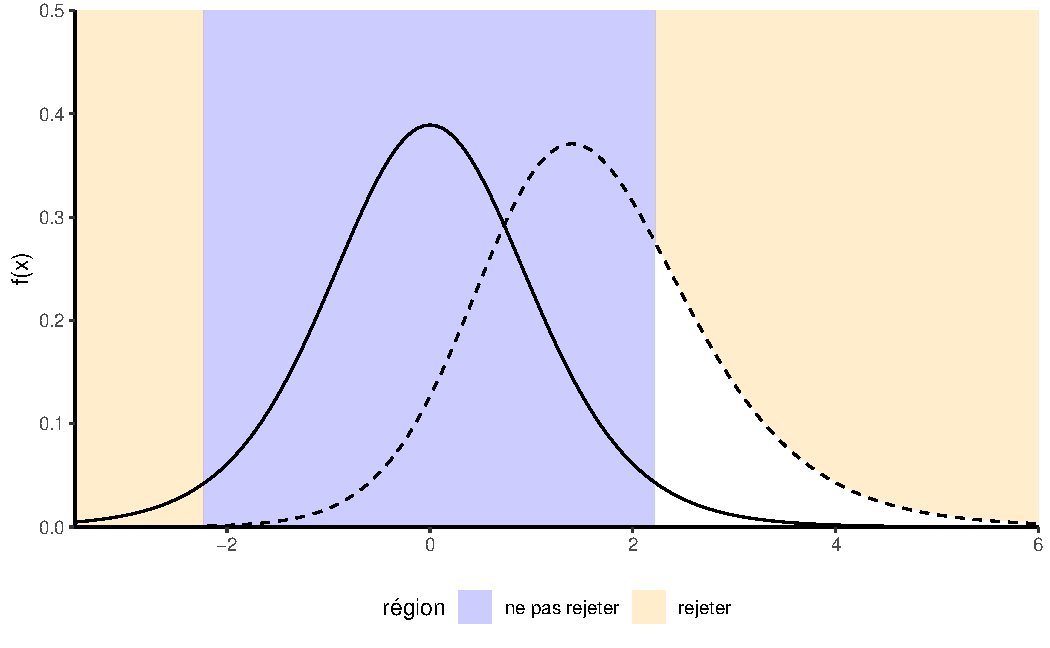
\includegraphics[width=0.85\textwidth,height=\textheight]{inference_files/figure-pdf/fig-puissance1-1.pdf}

}

\caption{\label{fig-puissance1}Comparaison de la loi nulle (ligne
pleine) et d'une alternative spécifique pour un test-\(t\) (ligne
traitillée). La puissance correspond à l'aire sous la courbe de la
densité de la loi alternative qui est dans la zone de rejet du test (en
blanc).}

\end{figure}%

\begin{figure}[ht!]

\centering{

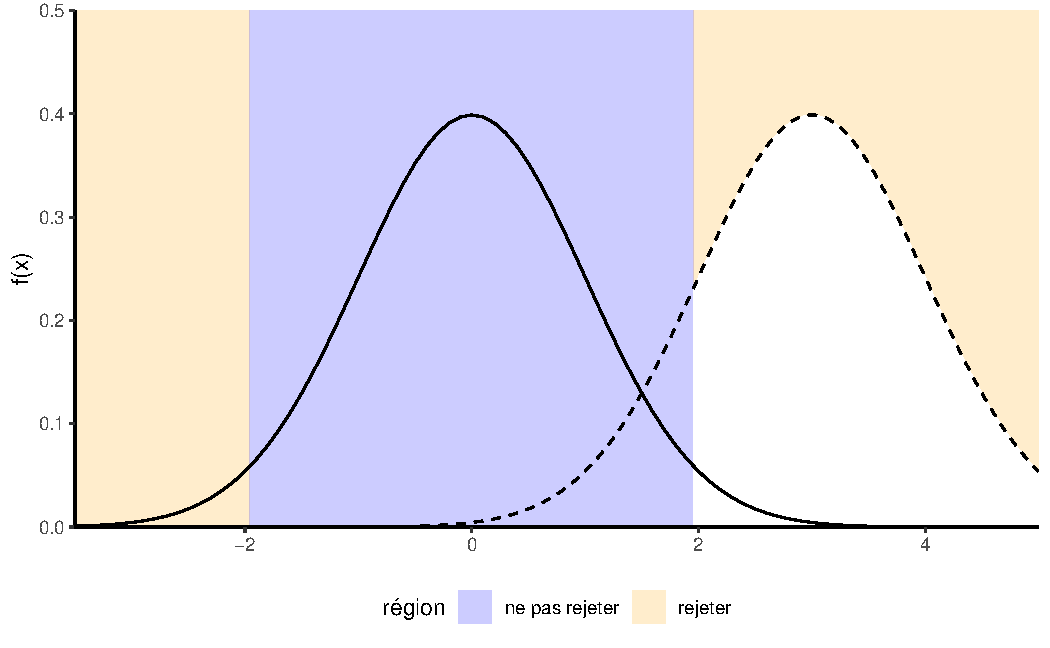
\includegraphics[width=0.85\textwidth,height=\textheight]{inference_files/figure-pdf/fig-puissance2-1.pdf}

}

\caption{\label{fig-puissance2}Augmentation de la puissance suite à une
augmentation de la différence de moyenne sous l'hypothèse alternative.
La puissance est l'aire sous la courbe (blanc) de la loi alternative
(ligne traitillée); cette dernière est plus décalée vers la droite par
rapport à la loi nulle postulée (ligne pleine).}

\end{figure}%

\begin{figure}[ht!]

\centering{

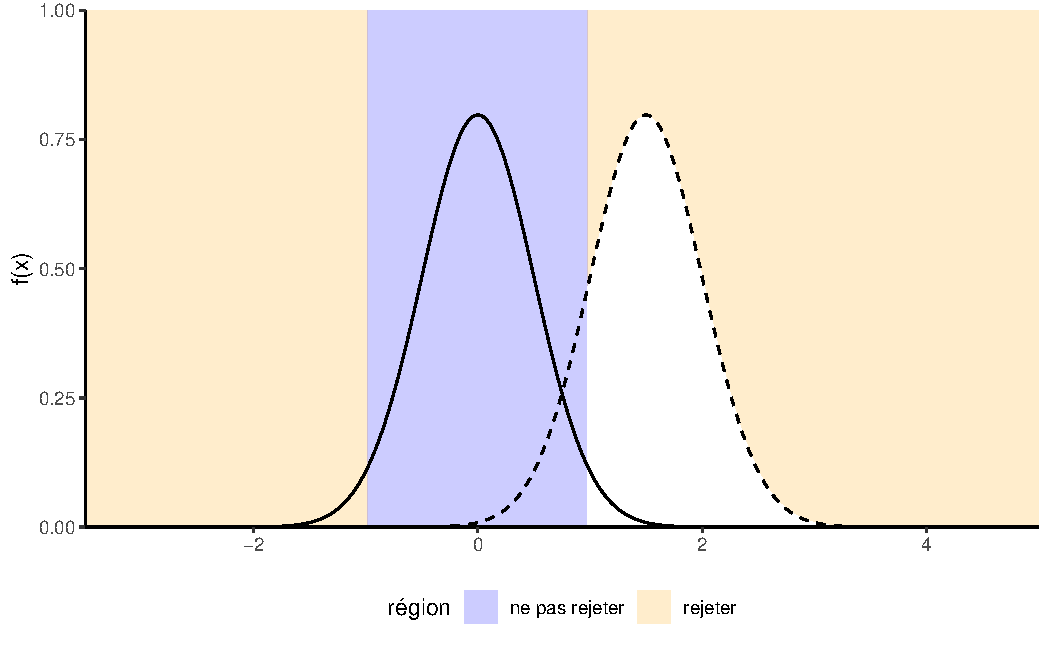
\includegraphics[width=0.85\textwidth,height=\textheight]{inference_files/figure-pdf/fig-puissance3-1.pdf}

}

\caption{\label{fig-puissance3}Augmentation de la puissance suite à une
augmentation de la taille de l'échantillon ou une diminution de
l'écart-type de la population: la loi nulle (ligne pleine) est plus
concentrée et la taille de la région de rejet diminue. La puissance est
l'aire sous la courbe (blanc) de la loi alternative (ligne traitillée).
Règle générale, la loi nulle change selon la taille de l'échantillon.}

\end{figure}%

On veut qu'un test ait une puissance élevée, c'est-à-dire, on veut que
\(\gamma\) soit le plus près de 1 possible. Minimalement, la puissance
du test devrait être \(\alpha\) si on rejette l'hypothèse nulle une
fraction \(\alpha\) du temps quand cette dernière est vraie. La
puissance dépend de plusieurs critères, à savoir:

\begin{itemize}
\tightlist
\item
  la taille de l'effet: plus la différence est grande entre la valeur du
  paramètre postulé \(\theta_0\) sous \(\mathscr{H}_0\) et le
  comportement observé, plus il est facile de le détecter (voir
  Figure~\ref{fig-puissance3});
\item
  la variabilité: moins les observations sont variables, plus il est
  facile de déterminer que la différence observée est significative (les
  grandes différences sont alors moins plausibles, comme l'illustre la
  Figure~\ref{fig-puissance2});
\item
  la taille de l'échantillon: plus on a d'observations, plus notre
  capacité à détecter une différence significative augmente parce que
  l'erreur-type décroît avec la taille de l'échantillon à un rythme
  (ordinairement) de \(n^{-1/2}\). La loi nulle devient aussi plus
  concentrée quand la taille de l'échantillon augmente.
\item
  le choix de la statistique de test: par exemple, les statistiques
  basées sur les rangs n'utilisent pas les valeurs numériques qu'à
  travers le rang relatif. Ces tests sont donc moins puissants parce
  qu'ils n'utilisent pas toute l'information dans l'échantillon; en
  contrepartie, ils sont souvent plus robustes en présence de valeurs
  aberrantes et si le modèle est mal spécifié. Les statistiques de test
  que nous choisirons sont souvent standards et parmi les plus
  puissantes qui soient, aussi on ne traitera pas de ce point davantage
  dans le cadre du cours.
\end{itemize}

Pour calculer la puissance d'un test, il faut choisir une alternative
spécifique. Pour des exemples simples de statistiques, on peut obtenir
une formule pour la puissance: par exemple, si on utilise un test-\(t\)
pour un échantillon, la statistique
\(T=\sqrt{n}(\overline{X}-\mu_0)/S_n \sim \mathcal{T}_{n-1}\) et, si la
vraie moyenne est \(\Delta + \mu_0\), alors la loi alternative est
Student-\(t\), mais non-centrée avec paramètre de décalage \(\Delta\).
Cette dérivation est l'exception plutôt que la règle et on détermine
d'ordinaire la puissance à l'aide de méthodes de Monte Carlo en simulant
des observations d'une alternative donnée, en calculant la statistique
de test sur le nouvel échantillon simulé et en calculant la
valeur-\emph{p} associée à notre hypothèse nulle de façon répétée. On
calcule par la suite la proportion de tests qui mènent au rejet de
l'hypothèse nulle à niveau \(\alpha\), ce qui correspond au pourcentage
de valeurs-\(p\) inférieures à \(\alpha\).

\section{Intervalle de confiance}\label{intervalle-de-confiance}

Un \textbf{intervalle de confiance} est une manière alternative de
rapporter les conclusions d'un test, en ce sens qu'on fournit une
estimation ponctuelle de \(\hat{\theta}\) avec une marge d'erreur.
L'intervalle de confiance donne donc une indication de la variabilité de
la procédure d'estimation. Un intervalle de confiance de Wald à
\((1-\alpha)\) pour un paramètre \(\theta\) est de la forme
\begin{align*}
\widehat{\theta} \pm \mathfrak{q}_{\alpha/2} \; \mathrm{se}(\widehat{\theta})
\end{align*} où \(\mathfrak{q}_{\alpha/2}\) est le quantile d'ordre
\(1-\alpha/2\) de la loi nulle de la statistique de Wald, \begin{align*}
T =\frac{\widehat{\theta}-\theta}{\mathrm{se}(\widehat{\theta})},
\end{align*} et où \(\theta\) représente la valeur du paramètre
\(\theta\) (supposé fixe, mais inconnu) de la population. Les bornes de
l'intervalle de confiance sont aléatoires puisque \(\widehat{\theta}\)
et \(\mathrm{se}(\widehat{\theta})\) sont des variable aléatoires: leurs
valeurs observées changent d'un échantillon à un autre.

Par exemple, pour un échantillon aléatoire \(X_1, \ldots, X_n\)
provenant d'une loi normale \(\mathsf{Norm}(\mu, \sigma)\), l'intervalle
de confiance à \((1-\alpha)\) pour la moyenne (dans la population)
\(\mu\) est \begin{align*}
\overline{X} \pm t_{n-1, \alpha/2} \frac{S}{\sqrt{n}}
\end{align*} où \(t_{n-1, \alpha/2}\) est le quantile d'ordre
\(1-\alpha/2\) de la loi Student-\(t\) avec \(n-1\) degrés de libertés.

Avant qu'on calcule l'intervalle de confiance, il y a une probabilité de
\(1-\alpha\) que \(\theta\) soit contenu dans l'intervalle
\textbf{aléatoire} symmétrique
\((\widehat{\theta} - \mathfrak{q}_{\alpha/2} \; \mathrm{se}(\widehat{\theta}), \widehat{\theta} + \mathfrak{q}_{\alpha/2} \; \mathrm{se}(\widehat{\theta}))\),
où \(\widehat{\theta}\) dénote l'estimateur de \(\theta\). Une fois
qu'on obtient un échantillon et qu'on calcule les bornes de l'intervalle
de confiance, il n'y a plus de notion de probabilité: la vraie valeur du
paramètre \(\theta\) (inconnue) est soit contenue dans l'intervalle de
confiance, soit pas. La seule interprétation de l'intervalle de
confiance qui soit valable alors est la suivante: si on répète
l'expérience plusieurs fois et qu'à chaque fois on calcule un intervalle
de confiance à \(1-\alpha\), alors une proportion de \((1-\alpha)\) de
ces intervalles devraient contenir la vraie valeur de \(\theta\) (de la
même manière, si vous lancez une pièce de monnaie équilibrée, vous
devriez obtenir grosso modo une fréquence de 50\% de pile et 50\% de
face, mais chaque lancer donnera un ou l'autre de ces choix). Notre «
confiance » est dans la procédure et non pas dans les valeurs numériques
obtenues pour un échantillon donné.

\begin{figure}[ht!]

\centering{

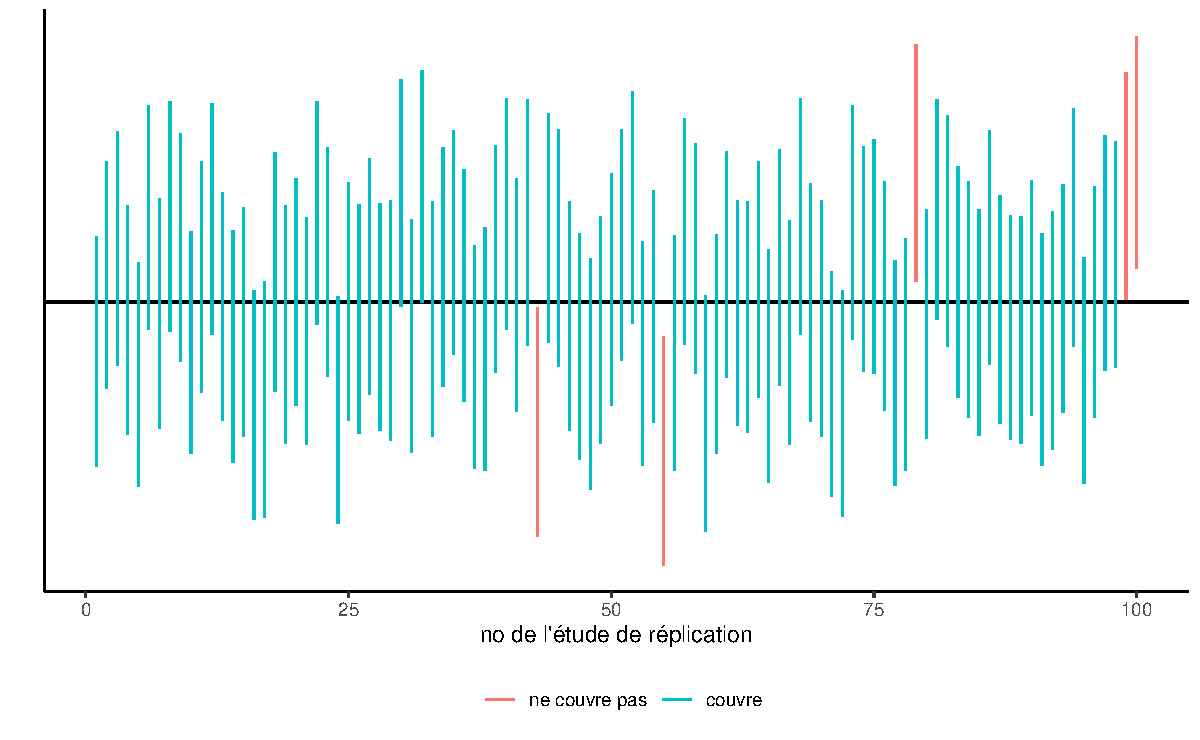
\includegraphics[width=0.85\textwidth,height=\textheight]{inference_files/figure-pdf/fig-intconf-1.pdf}

}

\caption{\label{fig-intconf}Intervalles de confiance à 95\% pour la
moyenne d'une population normale \(\mathsf{Norm}(0,1)\) pour 100
échantillons aléatoires. En moyenne, 5\% de ces intervalles (en rouge)
n'incluent pas la vraie valeur de la moyenne de zéro.}

\end{figure}%

Si on s'intéresse seulement à la décision rejeter/ne pas rejeter
\(\mathscr{H}_0\), l'intervalle de confiance est équivalent à la
valeur-\emph{p} en ce sens qu'il mène à la même décision. L'intervalle
de confiance donne en revanche l'ensemble des valeurs pour lesquelles la
statistique de test ne fournit pas assez de preuves pour rejeter
\(\mathscr{H}_0\): pour un test à niveau \(\alpha\), on ne rejetterait
aucune des valeurs contenues dans l'intervalle de confiance de niveau
\(1-\alpha\). Si la valeur-\emph{p} est inférieure à \(\alpha\), la
valeur postulée pour \(\theta\) est donc hors de l'intervalle de
confiance calculé. À l'inverse, la valeur-\emph{p} ne donne la
probabilité d'obtenir un résultat aussi extrême sous l'hypothèse nulle
que pour une seule valeur numérique, mais permet de quantifier
précisément à quel point le résultat est extrême.

\begin{example}[Achat en ligne de
milléniaux]\protect\hypertarget{exm-achats-milleniaux}{}\label{exm-achats-milleniaux}

Supposons qu'une chercheuse veut faire une étude sur l'évolution des
ventes en ligne au Canada. Elle postule que les membres de la génération
Y fait plus d'achats en ligne que ceux des générations antérieures. Pour
répondre à cette question, un sondage est envoyé à un échantillon
aléatoire de \(n=500\) individus représentatif de la population avec 160
membres de la génération Y et 340 personnes plus âgées. La variable
réponse est le montant d'achat effectués en ligne dans le mois dernier
(en dollars).

\end{example}

Dans cet exemple, on s'intéresse à la différence entre le montant moyen
des Y et celui des générations antérieures: la différence de moyenne
observée dans l'échantillon est de 16.49 dollars et donc les milléniaux
ont dépensé davantage. En revanche, notre échantillon est aléatoire et
le montant d'achat en ligne varie d'un individu à l'autre (et d'un mois
à l'autre): ce n'est donc pas suffisant pour dire que la différence est
significative.

La première étape de notre analyse consiste à définir les quantités
d'intérêt et à formuler nos hypothèse en fonction de paramètres du
modèle; il convient également de définir ces derniers en fonction des
variables en présence dans l'exemple. Ici, on considère un test pour la
différence de moyenne dans les populations postulées \(\mu_1\) (pour la
génération Y) et \(\mu_2\) (pour les générations antérieures)
d'écart-type respectif \(\sigma_1\) et \(\sigma_2\). Comment déterminer
quelle hypothèse on considère? Comme statisticien, on se fait l'avocat
du Diable: l'hypothèse d'intérêt du chercheur est l'hypothèse
alternative et ici, \(\mathscr{H}_a: \mu_1 > \mu_2\), où \(\mu_1\)
représente la moyenne des achats mensuels des milléniaux. L'hypothèse
nulle comprend toutes les autres valeurs pour la différence de moyenne,
soit \(\mathscr{H}_0: \mu_1 \leq \mu_2\). Il suffit néanmoins de
considérer le cas \(\mu_1=\mu_2\) (pourquoi?)

La deuxième étape consiste à choisir une statistique de test. S'il n'y a
aucune différence de moyenne entre les groupes, alors
\(\overline{X}_1-\overline{X}_2\) a moyenne zéro et la différence de
moyenne a une variance de \(\sigma^2_1/n_1+\sigma^2_2/n_2\). Ici, on
considère la statistique de Welch (\citeproc{ref-Welch:1947}{1947}) pour
une différence de moyenne entre deux échantillons: \begin{align*}
T = \frac{\overline{X}_1 - \overline{X}_2}{\left(\frac{S_1^2}{n_1}+\frac{S_2^2}{n_2} \right)^{1/2}}, \end{align*}
où \(\overline{X}_i\) est la moyenne empirique dans l'échantillon \(i\)
(\(i=1, 2\)) et \(S_i^2\) est la variance empirique et \(n_i\) la taille
de l'échantillon du groupe \(i\). La statistique est utilisée pour
calculer la différence de moyennes de deux échantillons de variance
potentiellement différente. La valeur de la statistique dans
l'échantillon est \(T=2.76\), mais on obtiendrait une valeur différente
avec un autre échantillon. Il convient donc de déterminer si cette
valeur est compatible avec notre hypothèse nulle en la comparant à la
loi nulle sous \(\mathscr{H}_0\) de \(T\). On effectuera le test à
niveau \(\alpha=0.05\).

La troisième étape est l'obtention d'un étalon de mesure pour déterminer
si notre résultat est extrême ou inattendu. Vous remarquerez que la
statistique de Welch a moyenne zéro et variance un sous l'hypothèse
nulle que \(\mu_1=\mu_2\): standardiser une statistique permet d'obtenir
un objet dont on connaît le comportement pour de grands échantillons et
obtenir une quantité sans unité de mesure. La dérivation de la loi nulle
est hors objectifs du cours, aussi cette dernière vous sera donnée dans
tous les cas qu'on considère. Asymptotiquement, \(T\) suit une loi
normale \(\mathsf{Norm}(0, 1)\), mais il existe une meilleure
approximation pour \(n\) petit; on compare le comportement de \(T\) à
l'aide d'une loi de Student via l'approximation de Satterthwaite
(\citeproc{ref-Satterthwaite:1946}{1946}).

La dernière étape consiste à obtenir une valeur-\emph{p}, soit la
probabilité d'observer un résultat aussi extrême sous \(\mathscr{H}_0\):
l'avantage de la valeur-\emph{p} est que cette valeur est une
probabilité (dans \([0, 1]\)) et qu'elle suit une loi uniforme sous
\(\mathscr{H}_0\). Puisque nous avons une hypothèse alternative
unilatérale, on regarde la probabilité sous \(\mathscr{H}_0\) que
\(\mathsf{Pr}(T > t)\). La valeur-\emph{p} vaut \(0.0031\) et donc, à
niveau 5\%, on rejette l'hypothèse nulle pour conclure que la génération
Y dépense davantage en ligne que les générations antérieures.

\begin{example}[Prix de billets de trains à grande vitesse
espagnols]\protect\hypertarget{exm-prix-trains-tests}{}\label{exm-prix-trains-tests}

La compagnie nationale de chemin de fer
\href{https://www.renfe.com/}{Renfe} gère les trains régionaux et les
trains à haute vitesse dans toute l'Espagne. Les prix des billets vendus
par Renfe sont
\href{https://www.kaggle.com/thegurusteam/spanish-high-speed-rail-system-ticket-pricing}{aggrégés}
par une compagnie. On s'intéresse ici à une seule ligne,
Madrid--Barcelone. Notre question scientifique est la suivante: est-ce
que le prix des billets pour un aller (une direction) est plus chère
pour un retour? Pour ce faire, on considère un échantillon de 10000
billets entre les deux plus grandes villes espagnoles. On s'intéresse au
billets de TGV vendus (AVE) au tarif Promotionnel. Notre statistique de
test sera simplement la différence de moyenne entre les deux
échantillons: la différence entre le prix en euros d'un train
Madrid--Barcelone (\(\mu_1\)) et le prix d'un billet Barcelone--Madrid
(\(\mu_2\)) est \(\mu_1-\mu_2\) et notre hypothèse nulle est qu'il n'y a
aucune différence de prix, soit \(\mathscr{H}_0: \mu_1-\mu_2=0\).

\end{example}

On utilise de nouveau le test de Welch pour deux échantillons en
filtrant les données pour ne conserver que les billets au tarif Promo:
la moyenne des billets Barcelone-Madrid est 82.11 euros, ceux pour
Madrid-Barcelone 82.56 euros et la valeur de la statistique de Welch est
-1.33. Si on utilise l'approximation normale, on obtient une
valeur-\emph{p} de 0.18.

Plutôt que d'utiliser la loi asymptotique (qui est valide pour de grands
échantillons à cause du théorème central limite), on peut considérer une
approximation sous une hypothèse moins restrictive en supposant que les
données sont échangeables. Sous l'hypothèse nulle, il n'y aucune
différence entre les deux destinations et les étiquettes pour la
destination (une variable catégorielle binaire) sont arbitraires. On
pourrait considérer les mêmes données, mais avec une permutation des
variables explicatives: c'est ce qu'on appelle un
\href{https://www.jwilber.me/permutationtest/}{test de permutation}. On
va recréer deux groupes de taille identique à notre échantillon
original, mais en changeant les observations. On recalcule la
statistique de test sur ces nouvelle données (si on a une poignée
d'observations, il est possible de lister toutes les permutations
possibles; typiquement, il suffit de considérer un grand nombre de
telles permutations, disons 9999). Pour chaque nouveau jeu de données,
on calculera la statistique de test et on calculera le rang de notre
statistique par rapport à cette référence. Si la valeur de notre
statistique observée sur l'échantillon original est extrême en
comparaison, c'est autant de preuves contre l'hypothèse nulle.

\begin{figure}[ht!]

\centering{

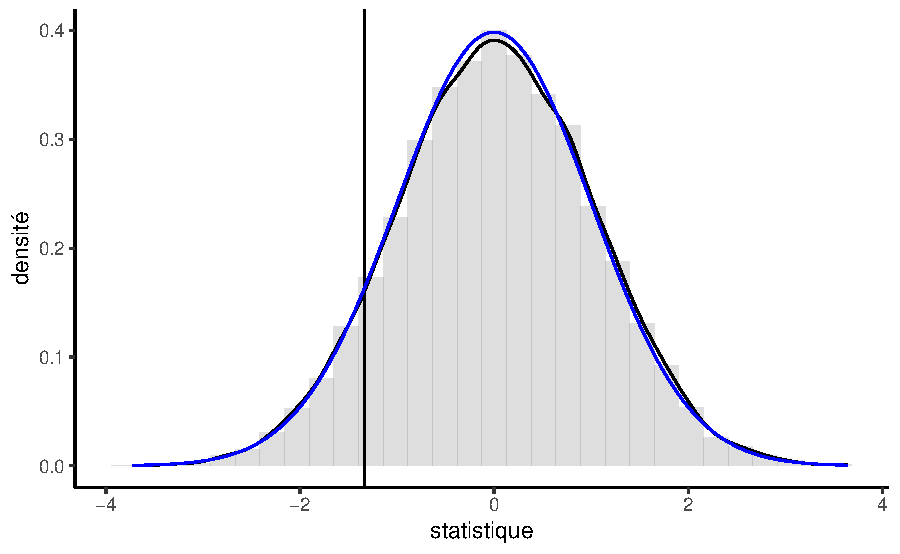
\includegraphics[width=0.85\textwidth,height=\textheight]{inference_files/figure-pdf/fig-renfepermut-1.pdf}

}

\caption{\label{fig-renfepermut}Approximation par permutation de la loi
nulle de la statistique de test de Welch (histogramme et trait noir) et
loi asymptotique normale standard (trait bleu) pour le prix de billets
de trains AVE au tarif promotionnel entre Madrid et Barcelone. La valeur
de la statistique de test de l'échantillon original est représentée par
un trait vertical.}

\end{figure}%

La valeur-\emph{p} du test de permutation, \(0.186\), est la proportion
de statistiques plus extrêmes que celle observée. Cette valeur-\emph{p}
est quasi-identique à celle de l'approximation de Satterthwaite, à
savoir \(0.182\) (la loi Student-\(t\) est numériquement équivalente à
une loi standard normale avec autant de degrés de liberté), tel que
représenté dans la Figure~\ref{fig-renfepermut}. Malgré que notre
échantillon soit très grand, avec \(n=8059\) observations, la différence
n'est pas jugée significative. Avec un échantillon de deux millions de
billets, on pourrait estimer précisément la moyenne (au centime près):
la différence de prix entre les deux destinations et cette dernière
deviendrait statistiquement significative. Elle n'est pas en revanche
pas pertinente en partique, car une différence de \(0.28\) euros sur un
prix moyen de \(82.56\) euros est quantité négligeable.

\bookmarksetup{startatroot}

\chapter*{Bibliographie}\label{bibliographie}
\addcontentsline{toc}{chapter}{Bibliographie}

\markboth{Bibliographie}{Bibliographie}

\phantomsection\label{refs}
\begin{CSLReferences}{1}{0}
\bibitem[\citeproctext]{ref-Brodeur:2021}
Brodeur, Mathieu, Perrine Ruer, Pierre-Majorique Léger, et Sylvain
Sénécal. 2021. {«~Smartwatches are more distracting than mobile phones
while driving: Results from an experimental study~»}. \emph{Accident
Analysis \& Prevention} 149: 105846.
\url{https://doi.org/10.1016/j.aap.2020.105846}.

\bibitem[\citeproctext]{ref-Brucks.Levav:2022}
Brucks, Melanie S., et Jonathan Levav. 2022. {«~Virtual communication
curbs creative idea generation~»}. \emph{Nature} 605 (7908): 108‑12.
\url{https://doi.org/10.1038/s41586-022-04643-y}.

\bibitem[\citeproctext]{ref-Duke.Amir:2023}
Duke, Kristen E., et On Amir. 2023. {«~The Importance of Selling
Formats: When Integrating Purchase and Quantity Decisions Increases
Sales~»}. \emph{Marketing Science} 42 (1): 87‑109.
\url{https://doi.org/10.1287/mksc.2022.1364}.

\bibitem[\citeproctext]{ref-Student:1908}
Gosset, William Sealy. 1908. {«~The probable error of a mean~»}.
\emph{Biometrika} 6 (1): 1‑25.
\url{https://doi.org/10.1093/biomet/6.1.1}.

\bibitem[\citeproctext]{ref-Lee.Choi:2019}
Lee, Kiljae, et Jungsil Choi. 2019. {«~Image-text inconsistency effect
on product evaluation in online retailing~»}. \emph{Journal of Retailing
and Consumer Services} 49: 279‑88.
\url{https://doi.org/10.1016/j.jretconser.2019.03.015}.

\bibitem[\citeproctext]{ref-McCullagh.Nelder:1989}
McCullagh, P., et J. A. Nelder. 1989. \emph{Generalized linear models}.
{S}econd edition. London: Chapman \& Hall.

\bibitem[\citeproctext]{ref-Moon.VanEpps:2023}
Moon, Alice, et Eric M VanEpps. 2023. {«~Giving Suggestions: Using
Quantity Requests to Increase Donations~»}. \emph{Journal of Consumer
Research} 50 (1): 190‑210. \url{https://doi.org/10.1093/jcr/ucac047}.

\bibitem[\citeproctext]{ref-Satterthwaite:1946}
Satterthwaite, F. E. 1946. {«~An Approximate Distribution of Estimates
of Variance Components~»}. \emph{Biometrics Bulletin} 2 (6): 110‑14.
\url{http://www.jstor.org/stable/3002019}.

\bibitem[\citeproctext]{ref-Sokolova:2023}
Sokolova, Tatiana, Aradhna Krishna, et Tim Döring. 2023. {«~Paper Meets
Plastic: The Perceived Environmental Friendliness of Product
Packaging~»}. \emph{Journal of Consumer Research} 50 (3): 468‑91.
\url{https://doi.org/10.1093/jcr/ucad008}.

\bibitem[\citeproctext]{ref-Welch:1947}
Welch, B. L. 1947. {«~The generalization of {``Student's''} problem when
several population variances are involved.~»} \emph{Biometrika} 34
(1--2): 28‑35. \url{https://doi.org/10.1093/biomet/34.1-2.28}.

\end{CSLReferences}


\backmatter


\end{document}
